\documentclass[11pt,a4paper]{article}
\usepackage{iftex}
\ifXeTeX
  \usepackage{fontspec}
\else
  \usepackage[utf8]{inputenc}
  \usepackage[T1]{fontenc}
  \usepackage{lmodern}
\fi
\usepackage[french]{babel}
\usepackage[margin=2.3cm]{geometry}
\usepackage{amsmath,amssymb}
\usepackage{graphicx}
\usepackage{booktabs,tabularx}
\usepackage{subcaption}
\usepackage{xcolor}
\usepackage{enumitem}
\usepackage{listings}
\usepackage{fancyhdr}
\usepackage{microtype}
\usepackage{hyperref}
\hypersetup{colorlinks=true,linkcolor=teal!60!black,urlcolor=teal!60!black,
 pdftitle={TP n° 2 — Localisation et scan matching},
 pdfauthor={Adib OUAMOU}}
\graphicspath{{figures/}}
\setlength{\parskip}{5pt}
\setlength{\parindent}{0pt}
\setlength{\emergencystretch}{2em}
\setlist[itemize]{nosep,leftmargin=*}
\pagestyle{fancy}
\fancyhf{}
\fancyhead[L]{TP n° 2 — Localisation LiDAR}
\fancyhead[R]{Adib OUAMOU}
\fancyfoot[C]{\thepage}
\setlength{\headheight}{14pt}
\lstset{basicstyle=\ttfamily\footnotesize,breaklines=true,
 frame=single,backgroundcolor=\color{gray!5},columns=fullflexible,
 keepspaces=true,showstringspaces=false}
\newcommand{\code}[1]{\texttt{\detokenize{#1}}}
\newcommand{\R}{\mathbb R}

\begin{document}
\pagenumbering{Alph}
\begin{titlepage}
\centering
\vspace*{1.8cm}
{\Large EIGSI\par}
\vspace{0.5cm}
{\large Cartographie et localisation appliquées à la robotique mobile\par}
\vspace{2cm}
{\Huge\bfseries Rapport de TP n° 2\par}
\vspace{0.7cm}
{\LARGE Localisation et scan matching\\à partir de mesures LiDAR\par}
\vspace{0.9cm}
{\large Cartes d'occupation, cartes vectorielles\\et recalage entre scans\par}
\vspace{0.6cm}
{\large\itshape Version améliorée\par}
\vfill
{\large Auteur\par}
\vspace{0.2cm}
{\LARGE\bfseries Adib OUAMOU\par}
\vspace{1cm}
{\large 3 novembre 2026 --- version améliorée du 4 novembre 2026\par}
\vspace{1cm}
\end{titlepage}

\pagenumbering{roman}
\begingroup
\setlength{\parskip}{0pt}
\tableofcontents
\endgroup
\newpage
\pagenumbering{arabic}

\section*{Introduction}
\addcontentsline{toc}{section}{Introduction}
Le TP n° 1 a permis d'acquérir des scans du LiDAR LD06 et de construire
des cartes d'occupation et des cartes vectorielles. Ce deuxième TP porte
sur la localisation : à partir d'un nouveau scan, il s'agit de retrouver
la position et l'orientation du capteur dans un repère de référence.

Trois types de référence sont étudiés : une grille d'occupation, un ensemble
de segments et un autre scan. Le minimum demandé est une méthode
fonctionnelle pour chacun, accompagnée d'une évaluation chiffrée.
Le travail compare quatre méthodes, dont deux pour le recalage entre scans,
en mesurant les erreurs de pose, le temps et le taux de réussite.

Il faut distinguer trois situations tout au long du rapport :
\begin{itemize}
\item une simulation avec des poses exactes connues et des scans calculés
par lancer de rayons depuis des positions différentes ;
\item des tests contrôlés sur des points réels, auxquels sont appliqués
des changements de repère connus ;
\item le recalage de deux acquisitions réelles, sans pose physique de
référence mesurée.
\end{itemize}
Ces situations n'ont pas la même portée. En particulier, un petit résidu
de recalage entre acquisitions réelles ne constitue pas une mesure de
l'erreur de position du robot.

\section{Données, repères et critères de localisation}
\subsection{Scans réels et conventions}
Les classeurs Scan 1, Scan 2 et Scan 3 contiennent chacun 454 impacts
valides après exclusion des distances nulles. Le classeur Fusion rassemble
5\,444 impacts issus de douze acquisitions, dont les poses ont été estimées
par recalage au TP précédent. Un nuage fusionné n'est pas assimilé à un
scan provenant d'une origine unique.

Les points locaux sont exprimés en mètres :
\[
 x=\frac{x_{\mathrm{lib}}}{1000},\qquad
 y=-\frac{y_{\mathrm{lib}}}{1000}.
\]
Une pose $\xi=(t_x,t_y,\theta)$ transforme le scan requête dans le repère
de la référence :
\[
 T_\xi(\mathbf p)=R(\theta)\mathbf p+\mathbf t,\qquad
 R(\theta)=
 \begin{pmatrix}\cos\theta&-\sin\theta\\\sin\theta&\cos\theta\end{pmatrix}.
\]
Les angles d'entrée et de sortie sont en degrés antihoraires. La rotation
est appliquée avant la translation.

\subsection{Condition de recouvrement}
La requête doit observer une zone représentée par la référence. Pour un
recalage entre scans, les acquisitions doivent être réalisées à des positions
proches et présenter suffisamment de surfaces communes. Les symétries,
les obstacles masqués ou déplacés et l'absence de recouvrement peuvent
rendre la pose ambiguë.

Le recouvrement numérique utilisé comme diagnostic est la proportion des
points à moins de 20 cm de la référence après transformation. Une valeur
inférieure à 50\,\% est signalée comme insuffisante. Ce seuil ne prouve
ni la validité physique d'une pose ni une couverture géométrique complète.

\subsection{Fonction de coût commune}
Pour une référence $\mathcal M$, la recherche minimise :
\[
 E(\xi)=\frac1N\sum_{i=1}^{N}
 \min\!\left(d\bigl(T_\xi(\mathbf p_i),\mathcal M\bigr),d_{\max}\right)^2,
 \qquad d_{\max}=0{,}60\ \mathrm m.
\]
La distance $d$ dépend du type de référence. La borne limite l'influence
des points très éloignés. Le coût RMS est la racine carrée de ce score ;
ce résidu borné ne doit pas être confondu avec l'erreur de pose.

\section{Localisation sur carte d'occupation}
\subsection{Champ de distance}
Le module \code{localisation_grid.py} charge une carte au format NPZ
produite par l'outil du TP n° 1. Les cellules occupées définissent les
obstacles. Une transformée de distance euclidienne calcule, pour chaque
cellule, la distance à la cellule occupée la plus proche.

Pour chaque pose candidate, les points de la requête sont placés dans la
carte et les distances sont lues par interpolation bilinéaire. Les
coordonnées sont rapportées aux centres des cellules, en tenant compte
du demi-pas de discrétisation. Un point hors carte reçoit la pénalité
maximale de 0,60 m ; il n'est pas supprimé de la moyenne.
La carte reste inchangée pendant la localisation.

\subsection{Recherche de pose grossière puis fine}
La fenêtre par défaut est de $\pm2$ m sur chacun des axes et $\pm30^\circ$
autour de la pose initiale. La recherche utilise trois niveaux :
\begin{table}[h]
\centering
\caption{Paramètres de la recherche hiérarchique de poses.}
\begin{tabular}{lrr}
\toprule
Niveau & Pas de translation & Pas angulaire \\
\midrule
Grossier & 0,25 m & $5^\circ$ \\
Intermédiaire & 0,05 m & $1^\circ$ \\
Fin & 0,01 m & $0,2^\circ$ \\
\bottomrule
\end{tabular}
\end{table}

Huit candidats distincts en position ou en orientation sont conservés entre
niveaux afin de ne pas raffiner uniquement des voisins immédiats du même
minimum grossier. Il s'agit d'une recherche hiérarchique dans l'espace des
poses, avec un champ de distance à résolution fixe, et non d'une pyramide
de grilles ni d'une recherche exhaustive à la résolution finale.
Une pose vraie hors fenêtre ne peut pas être retrouvée par cette recherche.

\subsection{Évaluation exploratoire sur les quatre jeux}
Une première campagne utilise 80\,\% des points pour la référence et
20\,\% pour le test, avec cinq transformations imposées. Pour les scans
individuels, cela représente 363 points de référence et 91 points de test.
Pour Fusion, la référence conserve les origines des douze acquisitions ;
chaque requête provient d'une seule acquisition.

\begin{table}[h]
\centering
\caption{Localisation sur grille : campagne exploratoire à cinq cas.}
\begin{tabular}{lrrr}
\toprule
Données & Erreur moyenne de position & Erreur angulaire & Réussites \\
\midrule
Scan 1 & 0,0293 m & $0,80^\circ$ & 5/5 \\
Scan 2 & 0,0508 m & $1,00^\circ$ & 5/5 \\
Scan 3 & 0,0242 m & $0,80^\circ$ & 5/5 \\
Fusion & 0,5227 m & $2,96^\circ$ & 2/5 \\
\bottomrule
\end{tabular}
\end{table}

Les échecs sur Fusion ne sont pas retirés des statistiques. Deux des cinq
requêtes n'atteignent que 15,4\,\% et 24,2\,\% de recouvrement à leur pose
imposée. Elles ne constituent donc pas une validation dans de bonnes
conditions de couverture. Une autre requête échoue également malgré un
recouvrement supérieur à 50\,\%. L'alignement des scans et les observations
contradictoires de la grille restent des points à examiner.

\section{Localisation sur carte vectorielle}
\subsection{Distance aux segments finis}
Le module \code{localisation_vectorielle.py} remplace le champ de distance
par une distance géométrique exacte aux segments de la carte. Pour un point
$\mathbf q$ et un segment $[\mathbf a,\mathbf b]$ :
\[
 \mathbf u=\mathbf b-\mathbf a,\qquad
 \lambda=\operatorname{clip}\left(
 \frac{(\mathbf q-\mathbf a)\cdot\mathbf u}{\|\mathbf u\|^2},0,1\right),
\]
\[
 d(\mathbf q,[\mathbf a,\mathbf b])
 =\|\mathbf q-(\mathbf a+\lambda\mathbf u)\|.
\]
La borne sur $\lambda$ impose une projection sur le segment fini, y compris
ses extrémités, et non sur sa droite infinie. La distance de référence est
le minimum sur tous les segments.

Le moteur de recherche de poses est identique à celui de la grille.
La référence n'est ni discrétisée en cellules ni échantillonnée en un
nuage de points. Tous les segments sont examinés par blocs afin de limiter
la mémoire.

\subsection{Référence construite sans les points de test}
Pour éviter une validation sur les mêmes impacts, les 20\,\% réservés sont
exclus \emph{avant} l'extraction et la consolidation des segments.
Les cartes de référence diffèrent donc des cartes du TP n° 1 calculées
avec tous les points. Elles contiennent respectivement 12, 5, 6 et
84 segments pour Scan 1, Scan 2, Scan 3 et Fusion.

\begin{table}[h]
\centering
\caption{Localisation vectorielle : campagne exploratoire à cinq cas.}
\begin{tabular}{lrrr}
\toprule
Données & Erreur moyenne de position & Erreur angulaire & Réussites \\
\midrule
Scan 1 & 0,0352 m & $0,40^\circ$ & 5/5 \\
Scan 2 & 0,0224 m & $0,00^\circ$ & 5/5 \\
Scan 3 & 0,0133 m & $0,40^\circ$ & 5/5 \\
Fusion & 0,0456 m & $0,40^\circ$ & 4/5 \\
\bottomrule
\end{tabular}
\end{table}

Sur Fusion, le premier cas atteint 0,1105 m d'erreur et dépasse le seuil
de 0,10 m. Le meilleur comportement vectoriel dans cette campagne ne prouve
pas l'exactitude de la carte : les segments peuvent conserver des surfaces
dédoublées qui restent compatibles avec les scans dont ils proviennent.
Les poses de base de Fusion demeurent des estimations.

\clearpage
\begin{figure}[p]
\centering
\begin{subfigure}{0.48\linewidth}
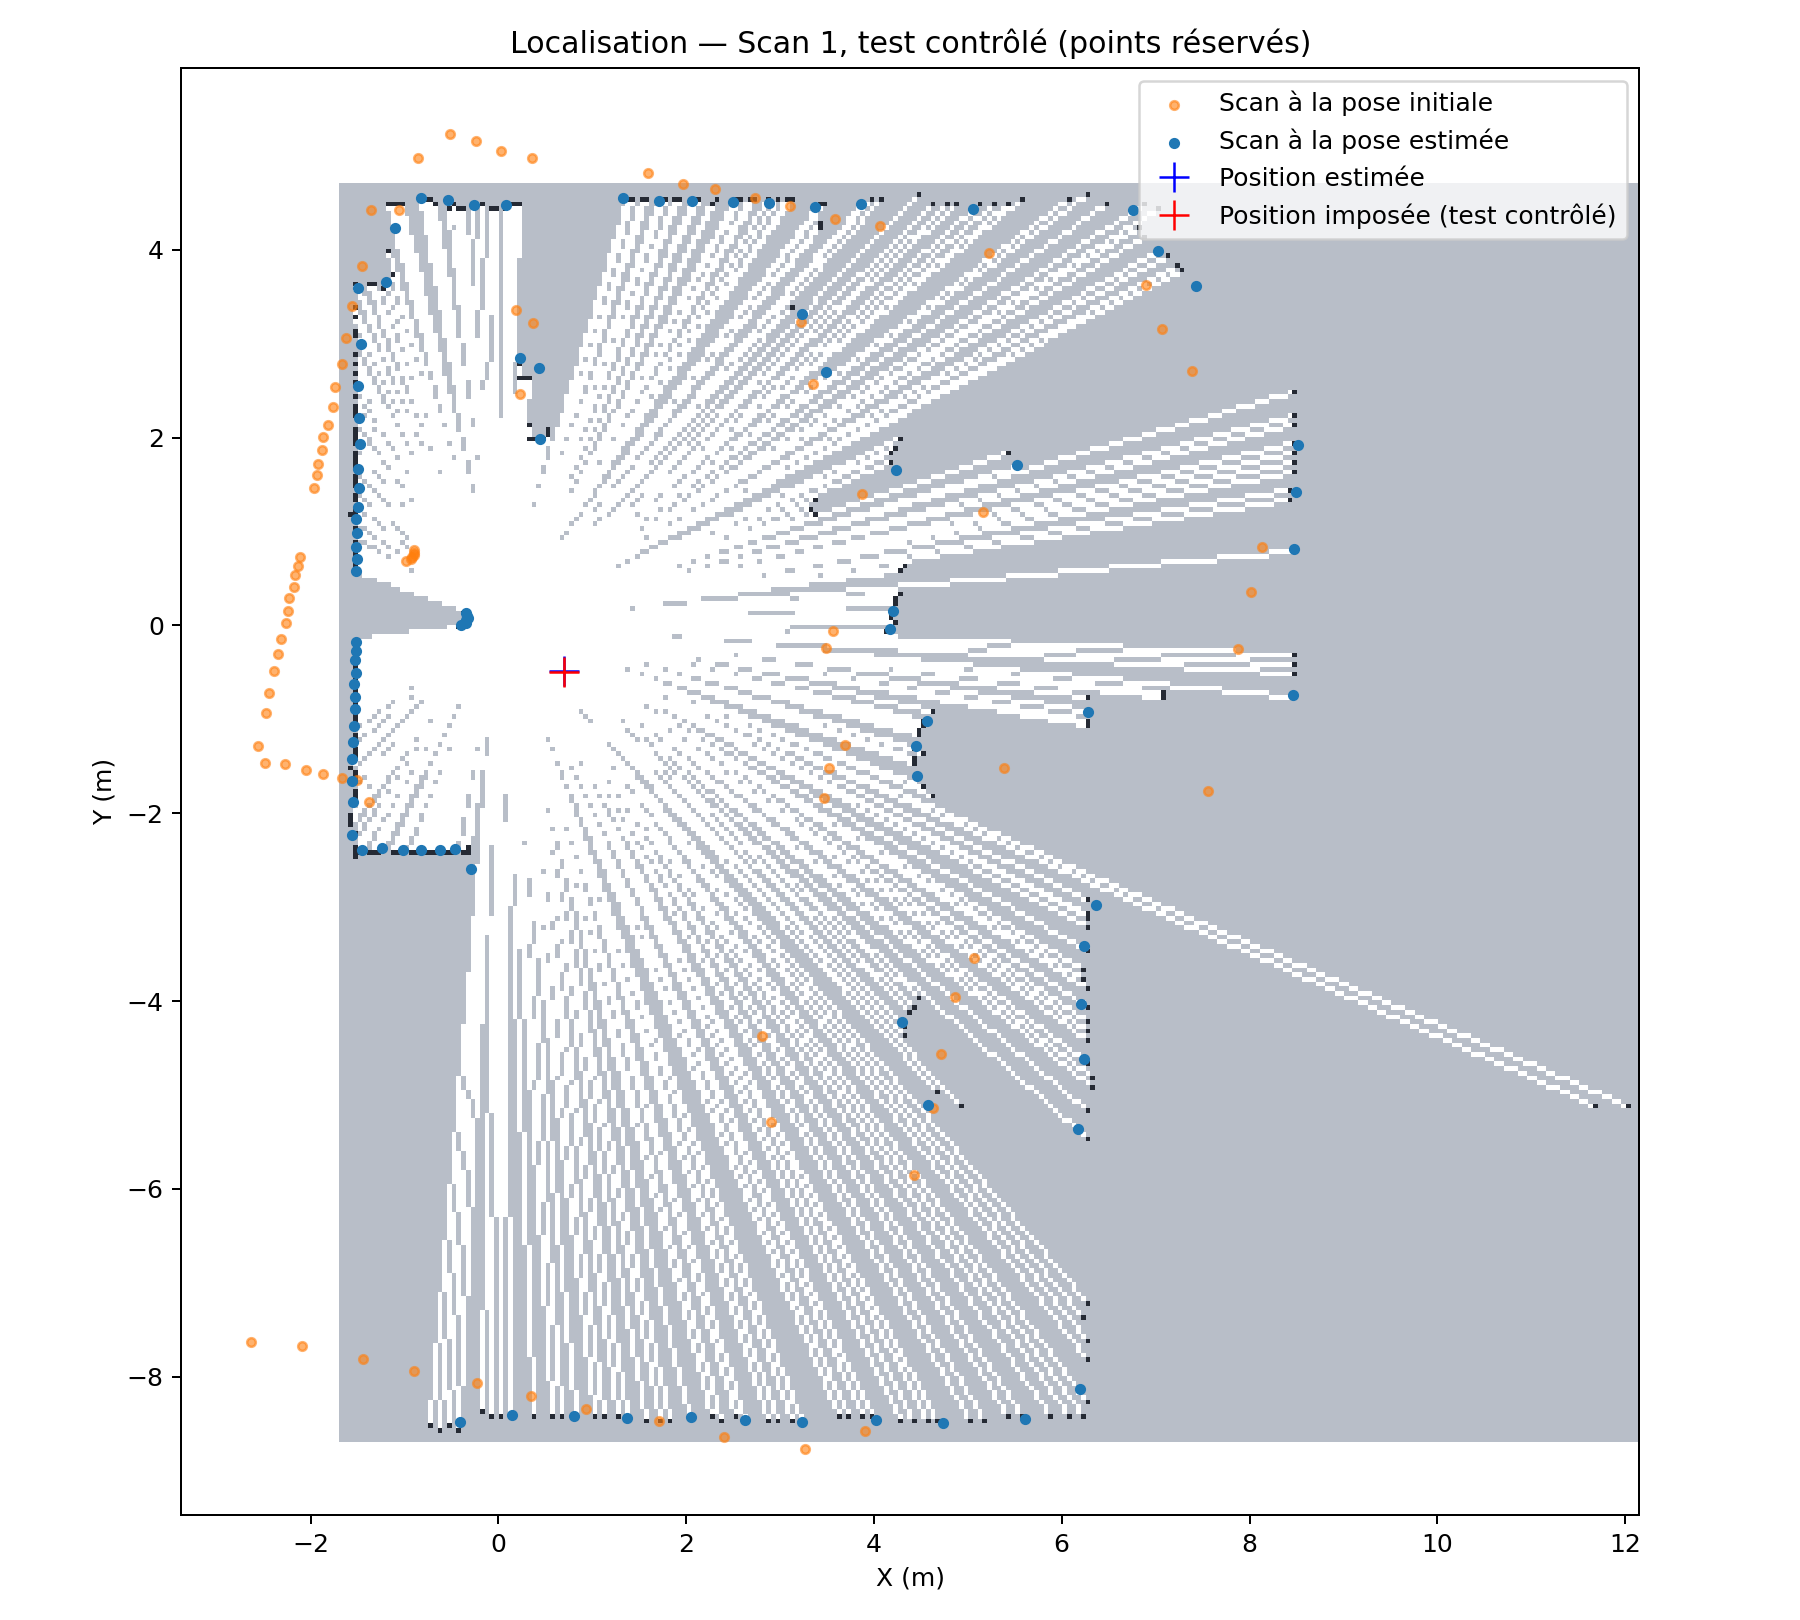
\includegraphics[width=\linewidth]{localisation_grid_scan_1.png}
\caption{Grille : Scan 1}
\end{subfigure}\hfill
\begin{subfigure}{0.48\linewidth}
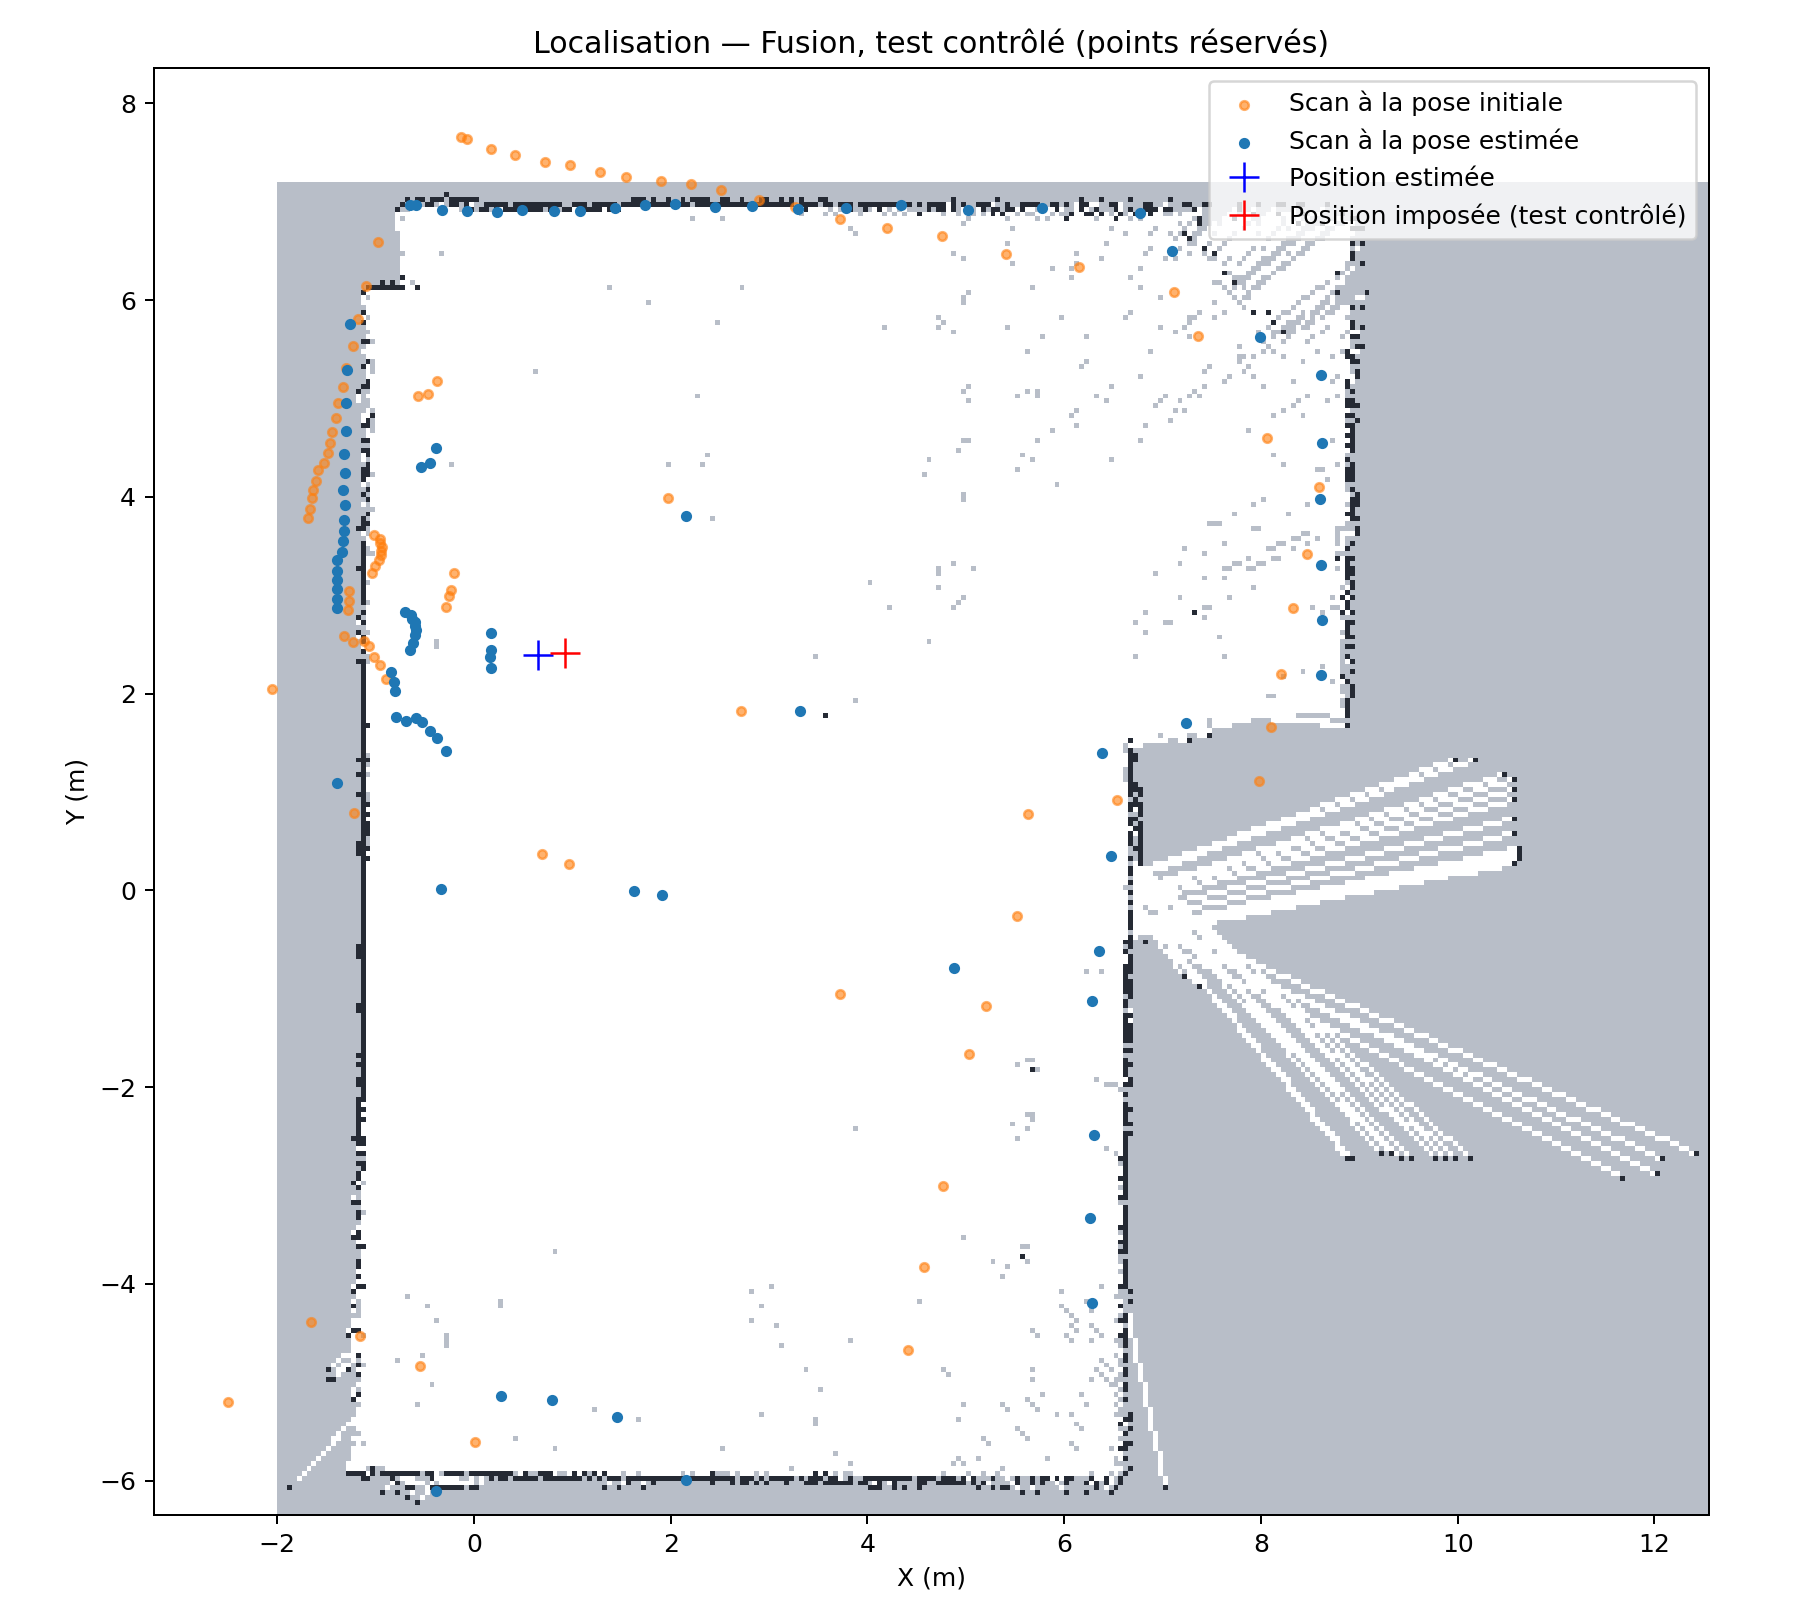
\includegraphics[width=\linewidth]{localisation_grid_fusion.png}
\caption{Grille : Fusion}
\end{subfigure}
\par\medskip
\begin{subfigure}{0.48\linewidth}
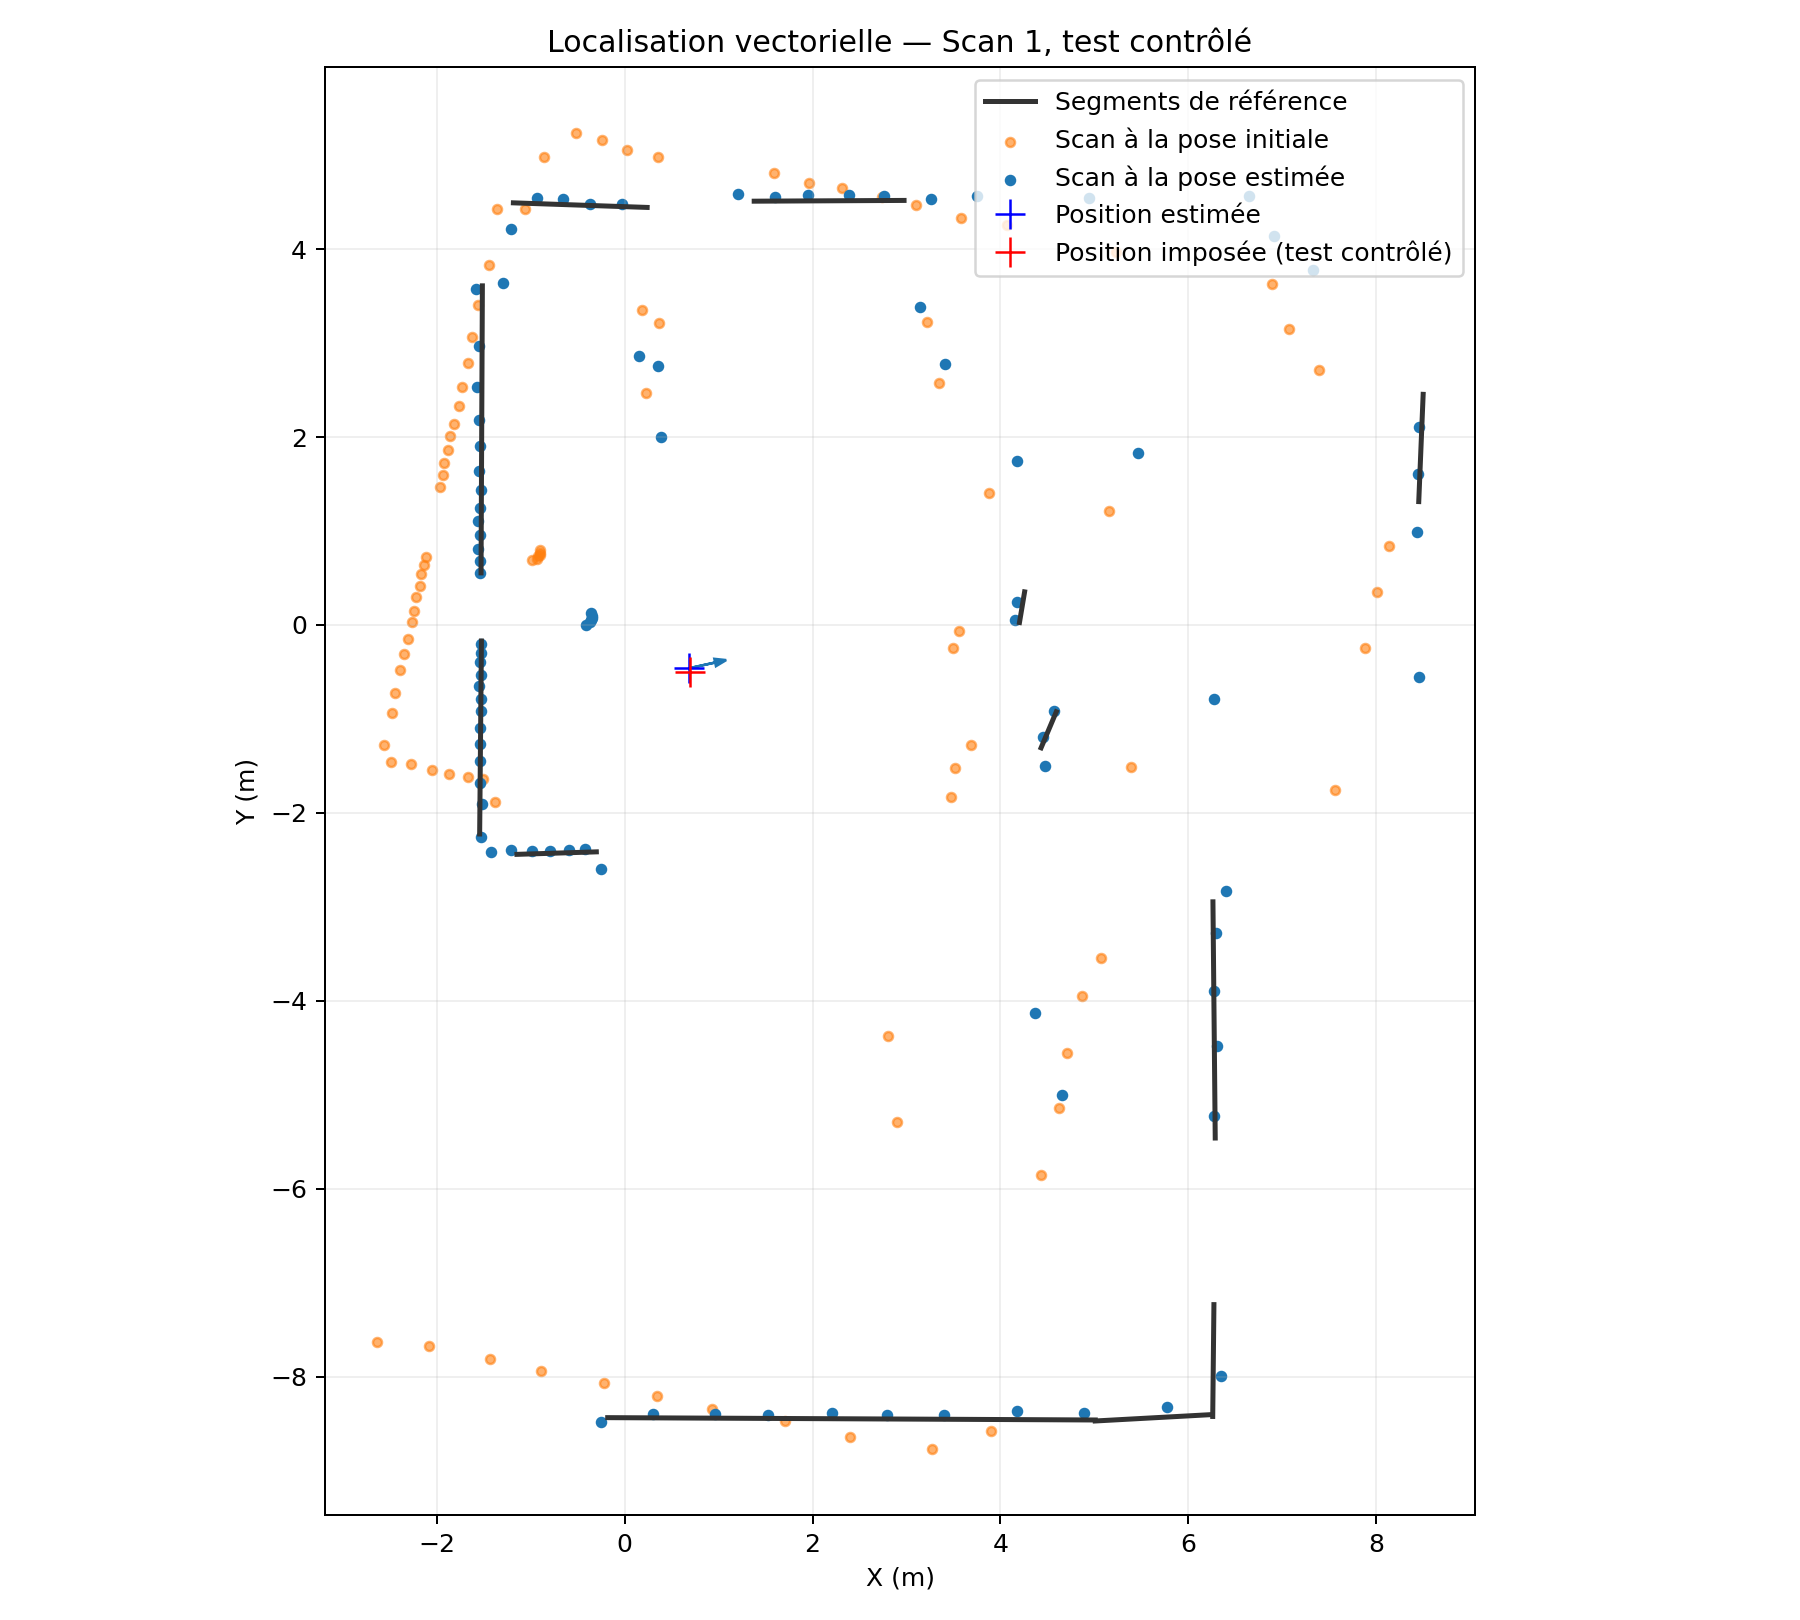
\includegraphics[width=\linewidth]{localisation_vectorielle_scan_1.png}
\caption{Segments : Scan 1}
\end{subfigure}\hfill
\begin{subfigure}{0.48\linewidth}
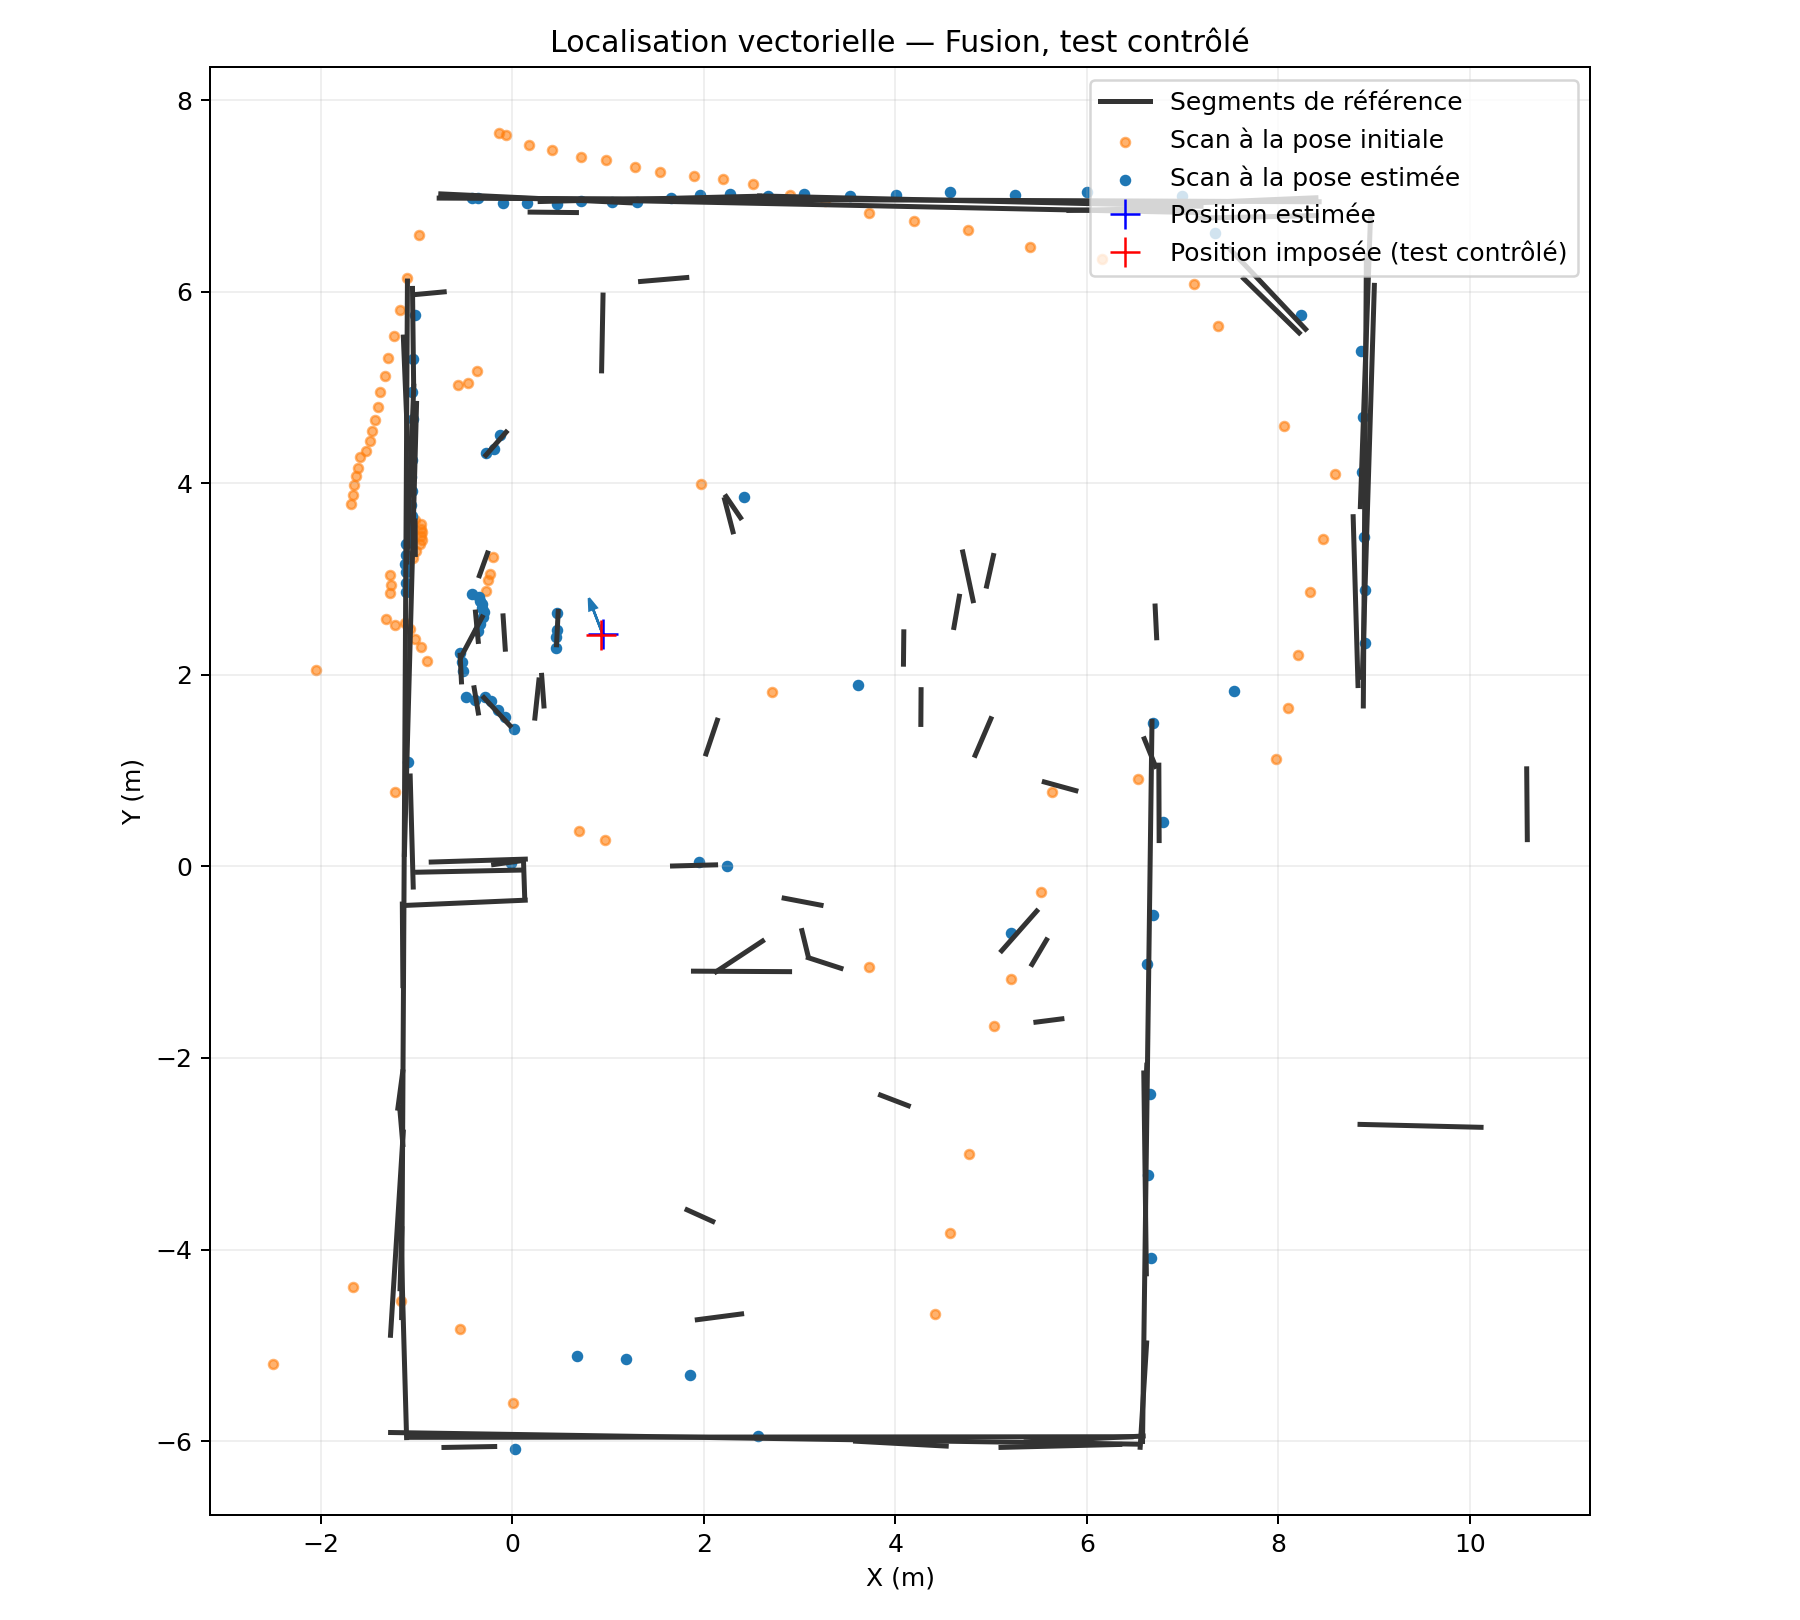
\includegraphics[width=\linewidth]{localisation_vectorielle_fusion.png}
\caption{Segments : Fusion}
\end{subfigure}
\caption{Exemples de localisation dans les campagnes contrôlées.
Orange : requête à la pose initiale ; bleu : requête à la pose estimée.
Les croix distinguent la position estimée et la position imposée de test.
La carte et les poses de base de Fusion restent estimées.}
\end{figure}
\clearpage

\section{Localisation entre scans}
\subsection{Recherche corrélative sur points}
Le module \code{localisation_scans.py} localise le scan requête dans le
repère d'un scan unique de référence. La classe \code{ScanMatcher}
construit un arbre KD des points de référence et calcule la distance au
plus proche voisin :
\[
 d(\mathbf q,\mathcal P_{\mathrm{ref}})
 =\min_{\mathbf r\in\mathcal P_{\mathrm{ref}}}\|\mathbf q-\mathbf r\|.
\]
La fonction de coût et les trois niveaux de recherche de pose sont ceux
des méthodes précédentes. Seule la représentation de la référence change.

\textbf{Version améliorée : distance point-à-ligne.} Chaque point de
référence reçoit la normale $\mathbf n_r$ du mur local, obtenue par analyse
en composantes principales de ses voisins à moins de 15 cm, lorsque ce
voisinage est rectiligne (rapport des écarts-types $\le 0{,}15$). La distance
devient l'écart le long de cette normale :
\[
 d(\mathbf q)=\bigl|\mathbf n_r^{\top}(\mathbf q-\mathbf r)\bigr|
 \quad\text{si } \|\mathbf q-\mathbf r\|\le 0{,}15\text{ m},
\]
et reste la distance point-à-point sinon (coins, objets isolés, points
éloignés de tout mur). La section~\ref{sec:amelioration} en donne l'effet mesuré.

\subsection{ICP en deux phases : point-à-point puis point-à-ligne}
Une deuxième méthode, \code{ICPMatcher}, affine directement la pose initiale
par ICP (\emph{Iterative Closest Point}). Dans la première phase, à chaque itération :
\begin{enumerate}[nosep]
\item Transformer les points du scan requête avec la pose courante.
\item Associer chaque point à son plus proche voisin dans la référence.
\item Exclure les correspondances à plus de 1,2 m et ne conserver que celles
dans les 80\,\% de distances les plus faibles.
\item Ajuster une rotation et une translation par moindres carrés/SVD,
sans réflexion.
\item Composer cette correction avec la transformation courante.
\end{enumerate}

Pour les correspondances retenues $(\mathbf q_i,\mathbf r_i)$, la correction
résout :
\[
 \min_{\Delta R,\Delta\mathbf t}
 \sum_i\|\Delta R\mathbf q_i+\Delta\mathbf t-\mathbf r_i\|^2,
 \qquad \det(\Delta R)=1.
\]
La translation est déduite des centres des ensembles après estimation
de la rotation. Les correspondances sont ensuite recalculées.

Au moins six correspondances sont requises. L'arrêt intervient après
80 itérations au maximum, ou lorsque la correction devient inférieure
à $10^{-5}$ m en translation et $10^{-3}$ degré en rotation.
L'ICP part uniquement de la pose initiale fournie ; aucune initialisation
globale cachée n'est utilisée dans la comparaison commune.

\textbf{Version améliorée : seconde phase point-à-ligne.} Après convergence
de la phase point-à-point, jusqu'à 30 itérations supplémentaires minimisent
la distance aux murs locaux, par un pas de Gauss-Newton linéarisé :
\[
 \min_{\delta x,\delta y,\delta\theta}\sum_i
 \Bigl(\mathbf n_i^{\top}\bigl(\mathbf q_i-\mathbf r_i
 +\delta\theta\,J\mathbf q_i+\delta\mathbf t\bigr)\Bigr)^2,
 \qquad J=\begin{pmatrix}0&-1\\1&0\end{pmatrix},
\]
sur les correspondances dotées d'une normale fiable (au moins 12).
Lancé seul, le point-à-ligne divergeait sur 5 essais sur 9 depuis les
initialisations éloignées : les points glissent le long des murs.
La phase point-à-point sert donc d'amorce robuste. Le résultat de la seconde
phase n'est conservé que s'il ne dégrade pas le coût borné ; sinon la pose
point-à-point est rendue.

Contrairement à la recherche de poses bornée, l'ICP n'est pas contraint
à rester dans la fenêtre $\pm2$ m/$\pm30^\circ$. Les sorties indiquent
s'il en sort. Son caractère local rend sa convergence dépendante de
l'initialisation et de la géométrie de la scène ; une convergence numérique
ne garantit pas une pose physique correcte.

\section{Protocole commun de comparaison}
Cette campagne, distincte des évaluations exploratoires à cinq cas,
compare les méthodes avec les mêmes requêtes et initialisations.

\subsection{Simulation à poses connues}
Le script \code{comparaison_localisation.py} crée une pièce de
$10\times8$ m contenant des obstacles asymétriques. Les scans sont calculés
par lancer de 450 rayons à $360^\circ$. Pour chaque rayon, seul le premier
impact visible est conservé. Un bruit radial gaussien indépendant d'écart-type
$\sigma=0{,}005$ m est ajouté, avec des graines fixées pour la reproduction.

Le scan de référence est acquis à la pose simulée $(0,0,0^\circ)$.
Les trois requêtes correspondent aux poses :
\[
 (0{,}7,-0{,}5,12^\circ),\quad
 (-0{,}8,0{,}6,-15^\circ),\quad
 (1{,}1,0{,}8,20^\circ).
\]
Elles sont situées à moins de 1,4 m de la référence. Il s'agit de scans
produits depuis des positions différentes, avec des occlusions et des
échantillonnages différents, et non de copies exactement superposables
du scan de référence. Un point de requête sur cinq est utilisé, soit
90 impacts par requête dans cette simulation.

Les poses sont exactes par construction dans le simulateur. Le bruit de
5 mm concerne les distances observées et non les coordonnées de vérité.
La référence est ensuite représentée sous forme de grille, de segments
ou de points à partir du \emph{même nuage de référence}.

\subsection{Expériences contrôlées sur les données réelles}
Pour chacun des trois scans réels individuels, les 363 points de référence
et les 91 points réservés sont séparés comme précédemment. Les points
réservés sont exprimés dans trois repères virtuels connus, avec les mêmes
transformations que celles indiquées pour la simulation.

Ce protocole vérifie la récupération géométrique d'une transformation sur
des données réelles, mais ne fournit pas trois nouveaux déplacements
physiquement mesurés du robot. Les résultats restent séparés de ceux de
la simulation dans les statistiques.

\subsection{Variation identique des poses initiales}
Pour chaque requête, trois décalages sont ajoutés à la pose connue pour
construire les initialisations de test :
\begin{table}[h]
\centering
\caption{Niveaux d'erreur initiale appliqués à toutes les méthodes.}
\begin{tabular}{lrrrr}
\toprule
Niveau & $\Delta X$ & $\Delta Y$ & $\Delta\theta$ & Erreur de position \\
\midrule
Proche & $+0,10$ m & $-0,10$ m & $+2^\circ$ & 0,14 m \\
Moyenne & $+0,80$ m & $-0,60$ m & $+15^\circ$ & 1,00 m \\
Difficile & $+1,50$ m & $-1,00$ m & $+25^\circ$ & 1,80 m \\
\bottomrule
\end{tabular}
\end{table}

La vérité sert à construire une expérience contrôlée et à évaluer les
erreurs. Elle n'est pas transmise au moteur de recalage. Pour chaque cas,
les quatre méthodes reçoivent exactement les mêmes points de requête
et la même initialisation. Toutes les poses vraies sont dans les fenêtres
des recherches hiérarchiques pour les niveaux choisis.

Au total, la campagne commune contient :
\[
 4\ \text{jeux}\times3\ \text{requêtes}\times
 3\ \text{initialisations}\times4\ \text{méthodes}
 =\boxed{144\ \text{essais}}.
\]

\subsection{Métriques et seuils de réussite}
Les métriques sont calculées après la localisation :
\[
 e_t=\|\widehat{\mathbf t}-\mathbf t^\star\|,\qquad
 e_\theta=
 \left|\operatorname{wrap}_{[-180^\circ,180^\circ)}
 \left(\widehat{\theta}-\theta^\star\right)\right|.
\]
Un essai est réussi si les \emph{deux} conditions sont satisfaites :
\[
 e_t\leq0{,}10\ \mathrm m,\qquad e_\theta\leq1^\circ.
\]
Le taux de réussite inclut tous les essais dans son dénominateur.
Le temps de recherche est mesuré séparément de la lecture et de la
préparation de la référence ; les temps de construction sont conservés
dans les métadonnées. Les durées dépendent du poste et de sa charge.

\section{Résultats de la comparaison commune}
\subsection{Résultats en simulation}
\begin{table}[h]
\centering
\caption{Simulation : neuf essais par méthode, trois poses et trois initialisations.}
\begin{tabular}{lrrrr}
\toprule
Méthode & $e_t$ moyen (m) & $e_\theta$ moyen & Temps moyen & Réussites \\
\midrule
Grille & 0,0245 & $0,533^\circ$ & 0,205 s & 9/9 \\
Vectorielle & 0,0133 & $0,267^\circ$ & 1,843 s & 9/9 \\
Recherche entre scans & 0,0080 & $0,267^\circ$ & 2,241 s & 9/9 \\
ICP entre scans & 0,0068 & $0,111^\circ$ & 0,035 s & 9/9 \\
\bottomrule
\end{tabular}
\end{table}

Sur cette scène et dans cette plage d'initialisation, toutes les méthodes
respectent les seuils. L'ICP est le plus rapide. Les recherches hiérarchiques
évaluent davantage de poses ; le champ de distance de la grille permet
un calcul de coût plus rapide que l'examen des segments ou des voisins
des points pour chaque pose candidate.

Ces observations ne démontrent pas qu'une méthode est toujours supérieure.
Le comportement peut changer avec une scène symétrique, un recouvrement
faible ou des initialisations plus éloignées.

\begin{figure}[htbp]
\centering
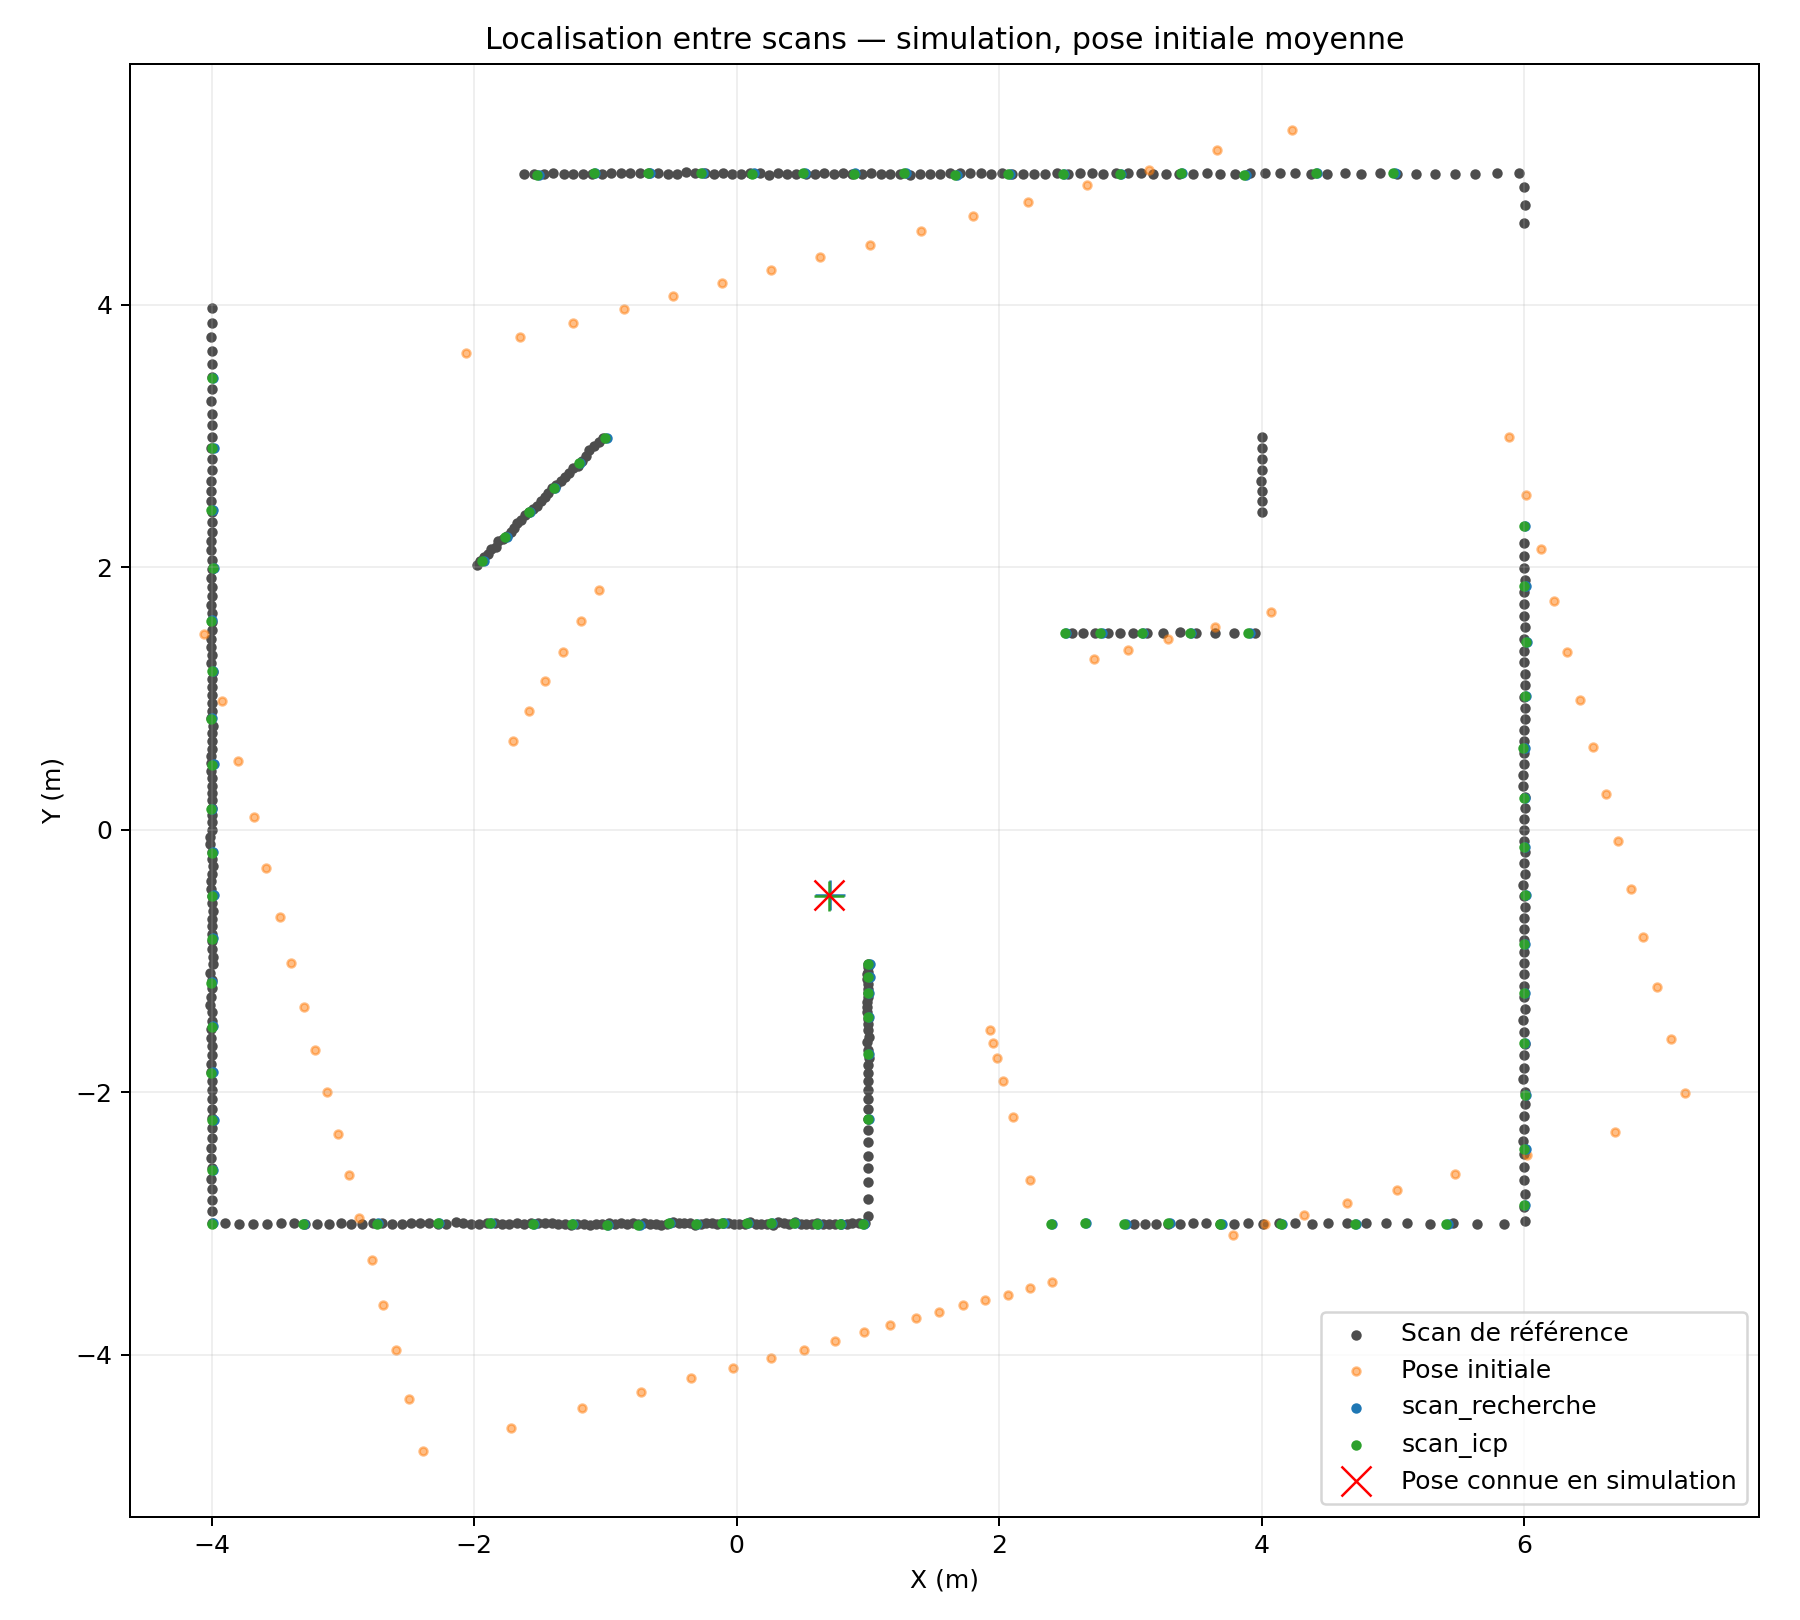
\includegraphics[width=0.75\linewidth]{comparaison_localisation_scans_simulation.png}
\caption{Recalage entre scans simulés, avec une initialisation moyenne.
Gris : référence ; orange : requête initiale ; bleu et vert :
requête après recherche et après ICP. La croix rouge indique la pose connue.}
\end{figure}

\subsection{Résultats sur les points réels réservés}
\begin{table}[htbp]
\centering
\caption{Erreurs moyennes de position en mètres, campagne commune.
Neuf essais par méthode et par scan.}
\begin{tabular}{lrrrr}
\toprule
Données & Grille & Vectorielle & Recherche scans & ICP scans \\
\midrule
Scan 1 & 0,0251 & 0,0407 & 0,0114 & 0,0158 \\
Scan 2 & 0,0559 & 0,0224 & 0,0551 & 0,0294 \\
Scan 3 & 0,0290 & 0,0114 & 0,0211 & 0,0270 \\
\bottomrule
\end{tabular}
\end{table}

\begin{table}[htbp]
\centering
\caption{Erreurs angulaires moyennes en degrés et temps moyens entre parenthèses,
en secondes, sur les points réels réservés.}
\begin{tabular}{lrrrr}
\toprule
Données & Grille & Vectorielle & Recherche scans & ICP scans \\
\midrule
Scan 1 & 0,800 (0,219) & 0,400 (2,395) & 0,600 (2,276) & 0,775 (0,068) \\
Scan 2 & 1,000 (0,236) & 0,000 (1,073) & 1,000 (2,693) & 0,808 (0,029) \\
Scan 3 & 0,800 (0,224) & 0,400 (1,154) & 0,800 (2,349) & 0,807 (0,034) \\
\bottomrule
\end{tabular}
\end{table}

Les quatre méthodes réussissent les neuf essais de chacun des trois scans
dans cette campagne. Ces chiffres portent sur des changements de repère
contrôlés d'une acquisition partagée en référence et test. Ils ne sont pas
des erreurs physiques mesurées lors d'un déplacement du robot. L'erreur
angulaire d'environ $0{,}8^\circ$ commune aux méthodes à base de points est
en grande partie un artefact de ce protocole (section~\ref{sec:amelioration}).

\subsection{Sensibilité observée à l'initialisation}
Dans les trois niveaux testés, les recherches hiérarchiques retrouvent les
mêmes poses finales pour un même jeu et une même requête. L'ICP présente
une légère augmentation de l'erreur sur certains scans réels lorsque
l'initialisation se dégrade, tout en restant sous les seuils retenus.

L'absence d'échec observé dans cette plage ne démontre pas une robustesse
globale. La pose vraie est toujours dans la fenêtre de recherche, les
scènes sont limitées et le bruit simulé reste modéré. Une campagne
supplémentaire pourrait tester des écarts hors fenêtre, plusieurs niveaux
de bruit et davantage de configurations symétriques.

\clearpage
\begin{figure}[p]
\centering
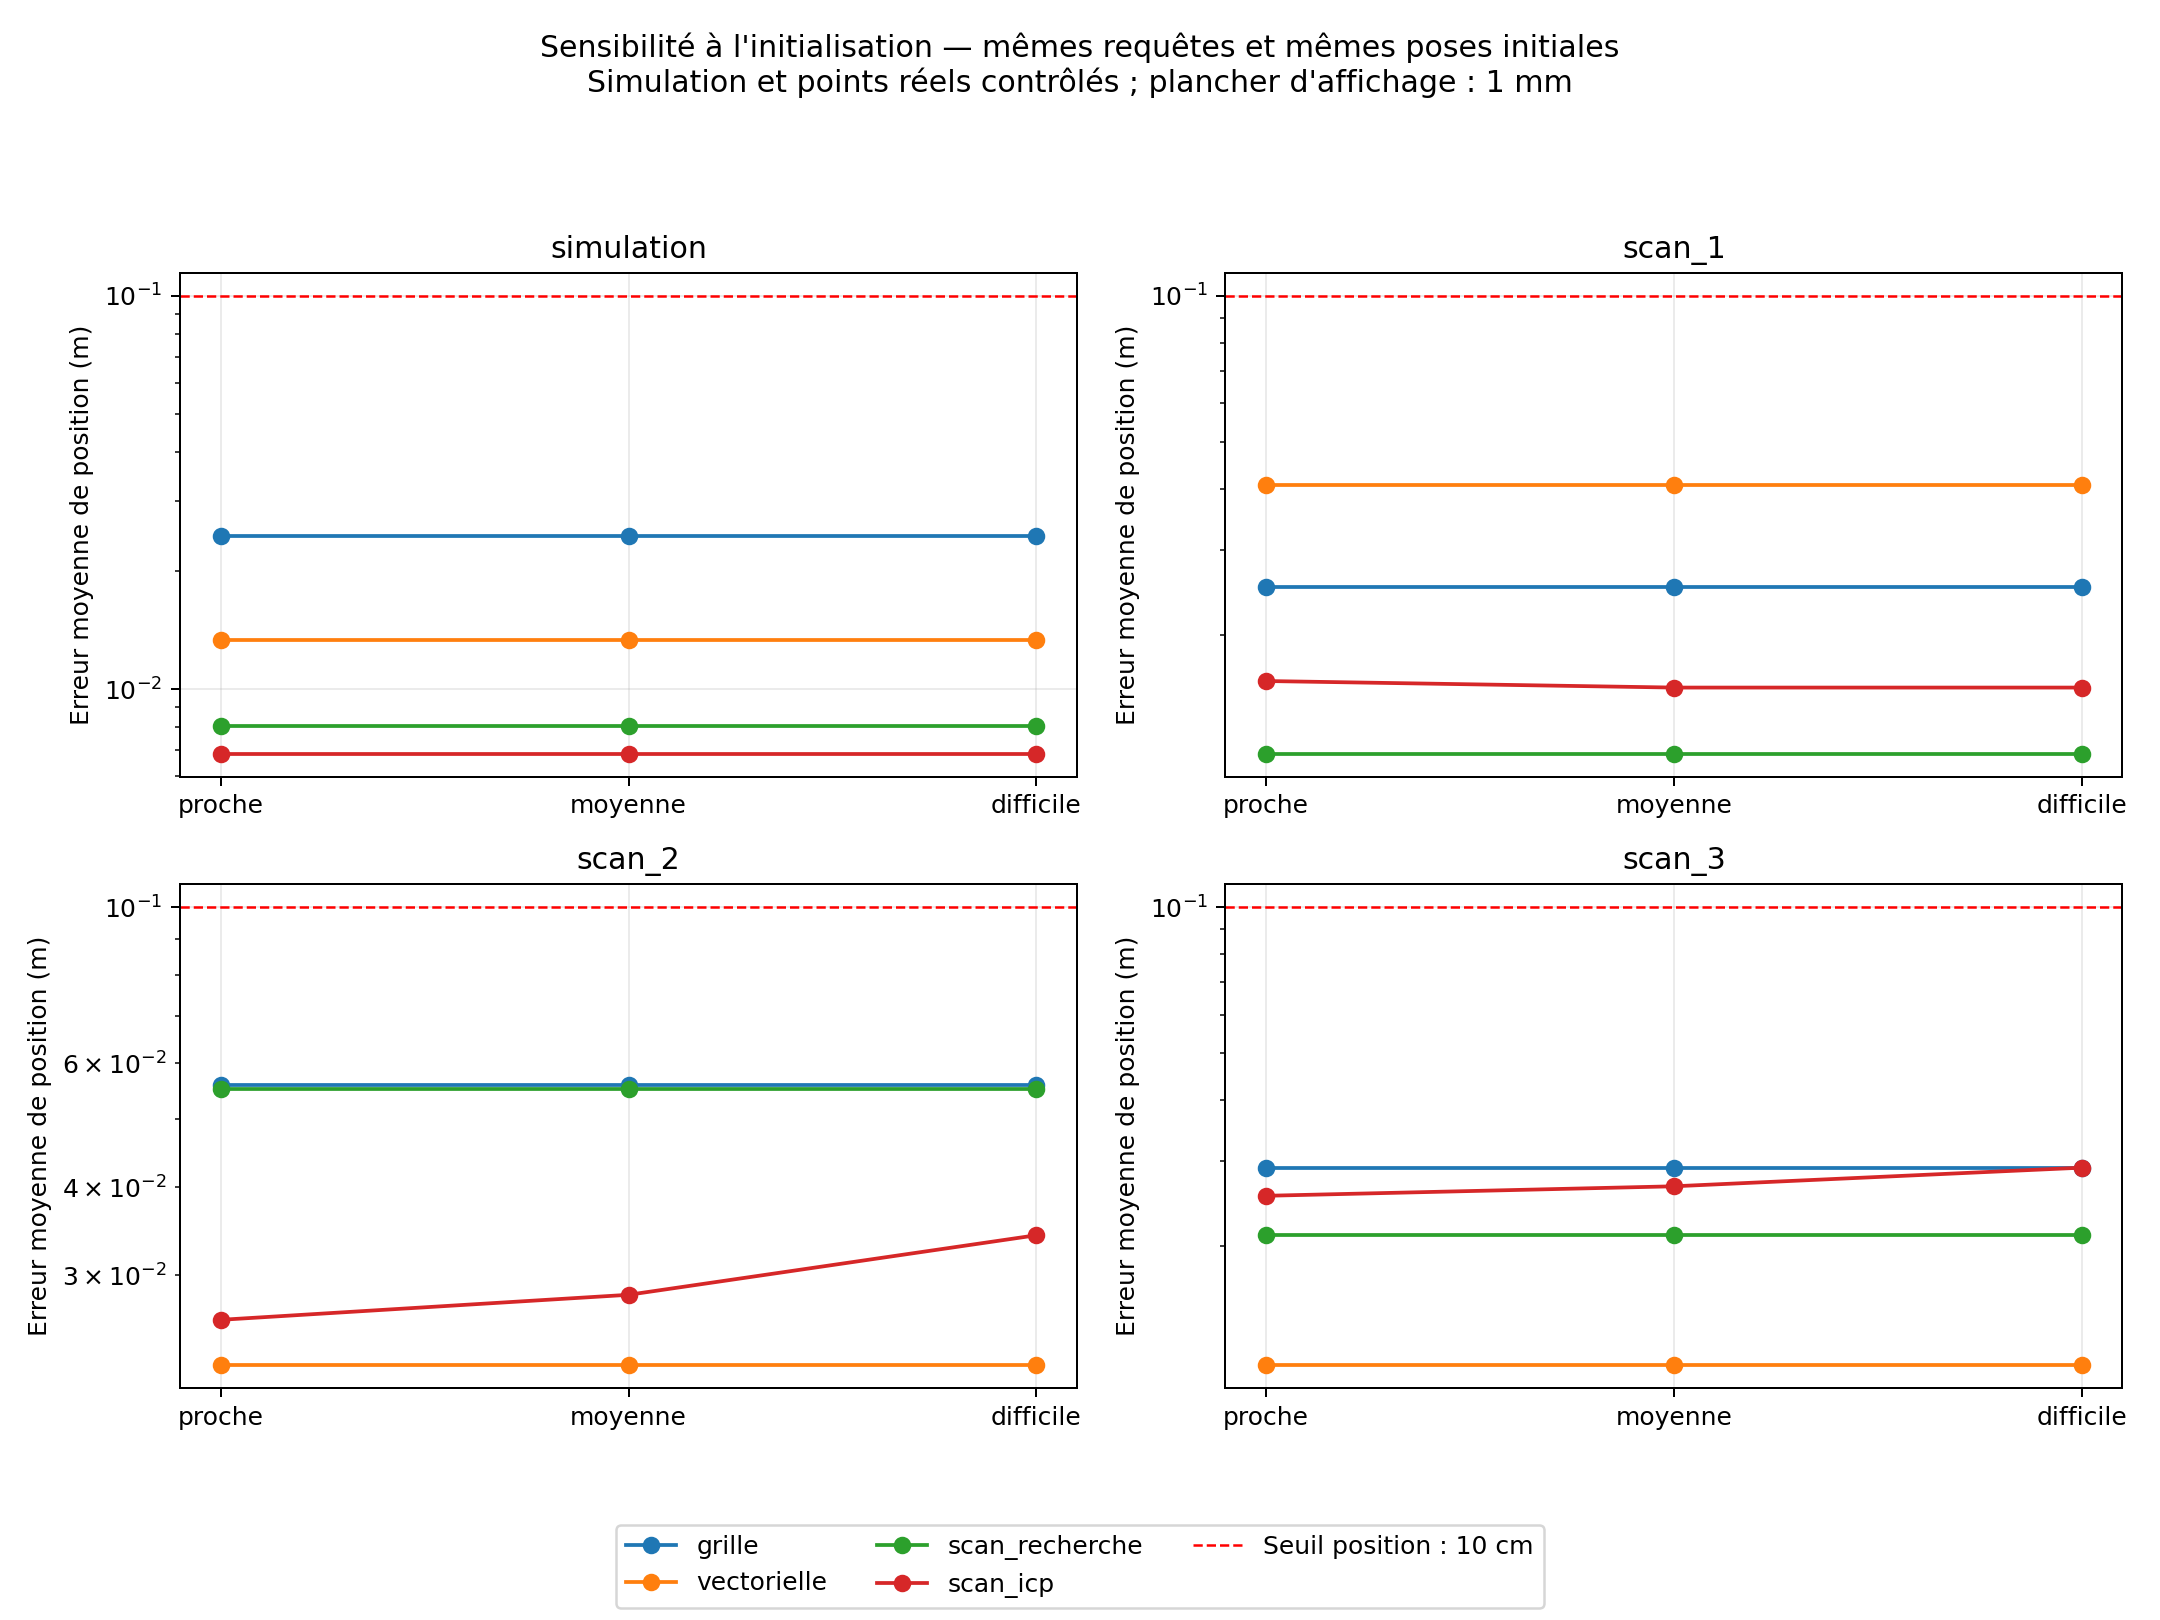
\includegraphics[width=\linewidth]{comparaison_localisation.png}
\caption{Sensibilité à l'initialisation : mêmes requêtes et mêmes poses
initiales pour toutes les méthodes. L'axe vertical représente l'erreur
moyenne de position sur une échelle logarithmique ; le seuil de 10 cm
est tracé en pointillés. La statistique angulaire et les temps sont
conservés séparément dans les CSV.}
\end{figure}
\clearpage

\section{Recalage des acquisitions réelles}
\subsection{Scan 3 dans le repère de Scan 2}
Un premier essai utilise Scan 2 comme référence et Scan 3 comme requête,
avec l'initialisation commune $(0,0,90^\circ)$. Cette valeur de $90^\circ$
est une approximation cohérente avec les rotations signalées pendant
l'acquisition, et non une orientation exactement mesurée entre ces fichiers.

\begin{table}[h]
\centering
\caption{Résultats estimés sur la paire réelle Scan 2/Scan 3.}
\begin{tabular}{lrrrr}
\toprule
Méthode & $X$ (m) & $Y$ (m) & Angle & Temps \\
\midrule
Recherche & 0,000 & 0,080 & $87,600^\circ$ & 11,979 s \\
ICP & 0,006 & 0,076 & $87,402^\circ$ & 0,035 s \\
\bottomrule
\end{tabular}
\end{table}

Les deux méthodes atteignent environ 99,8\,\% d'impacts à moins de 20 cm
de la référence. Les résidus RMS bornés sont respectivement de 0,053 m et
0,054 m. Dans la version d'origine, l'ICP point-à-point donnait
$88{,}205^\circ$ (résidu 0,063 m), à $0{,}6^\circ$ de la recherche ; les deux
méthodes indépendantes ne diffèrent plus que de $0{,}2^\circ$. Ils décrivent la cohérence géométrique des points, pas une erreur
de translation mesurée du robot.

\begin{figure}[htbp]
\centering
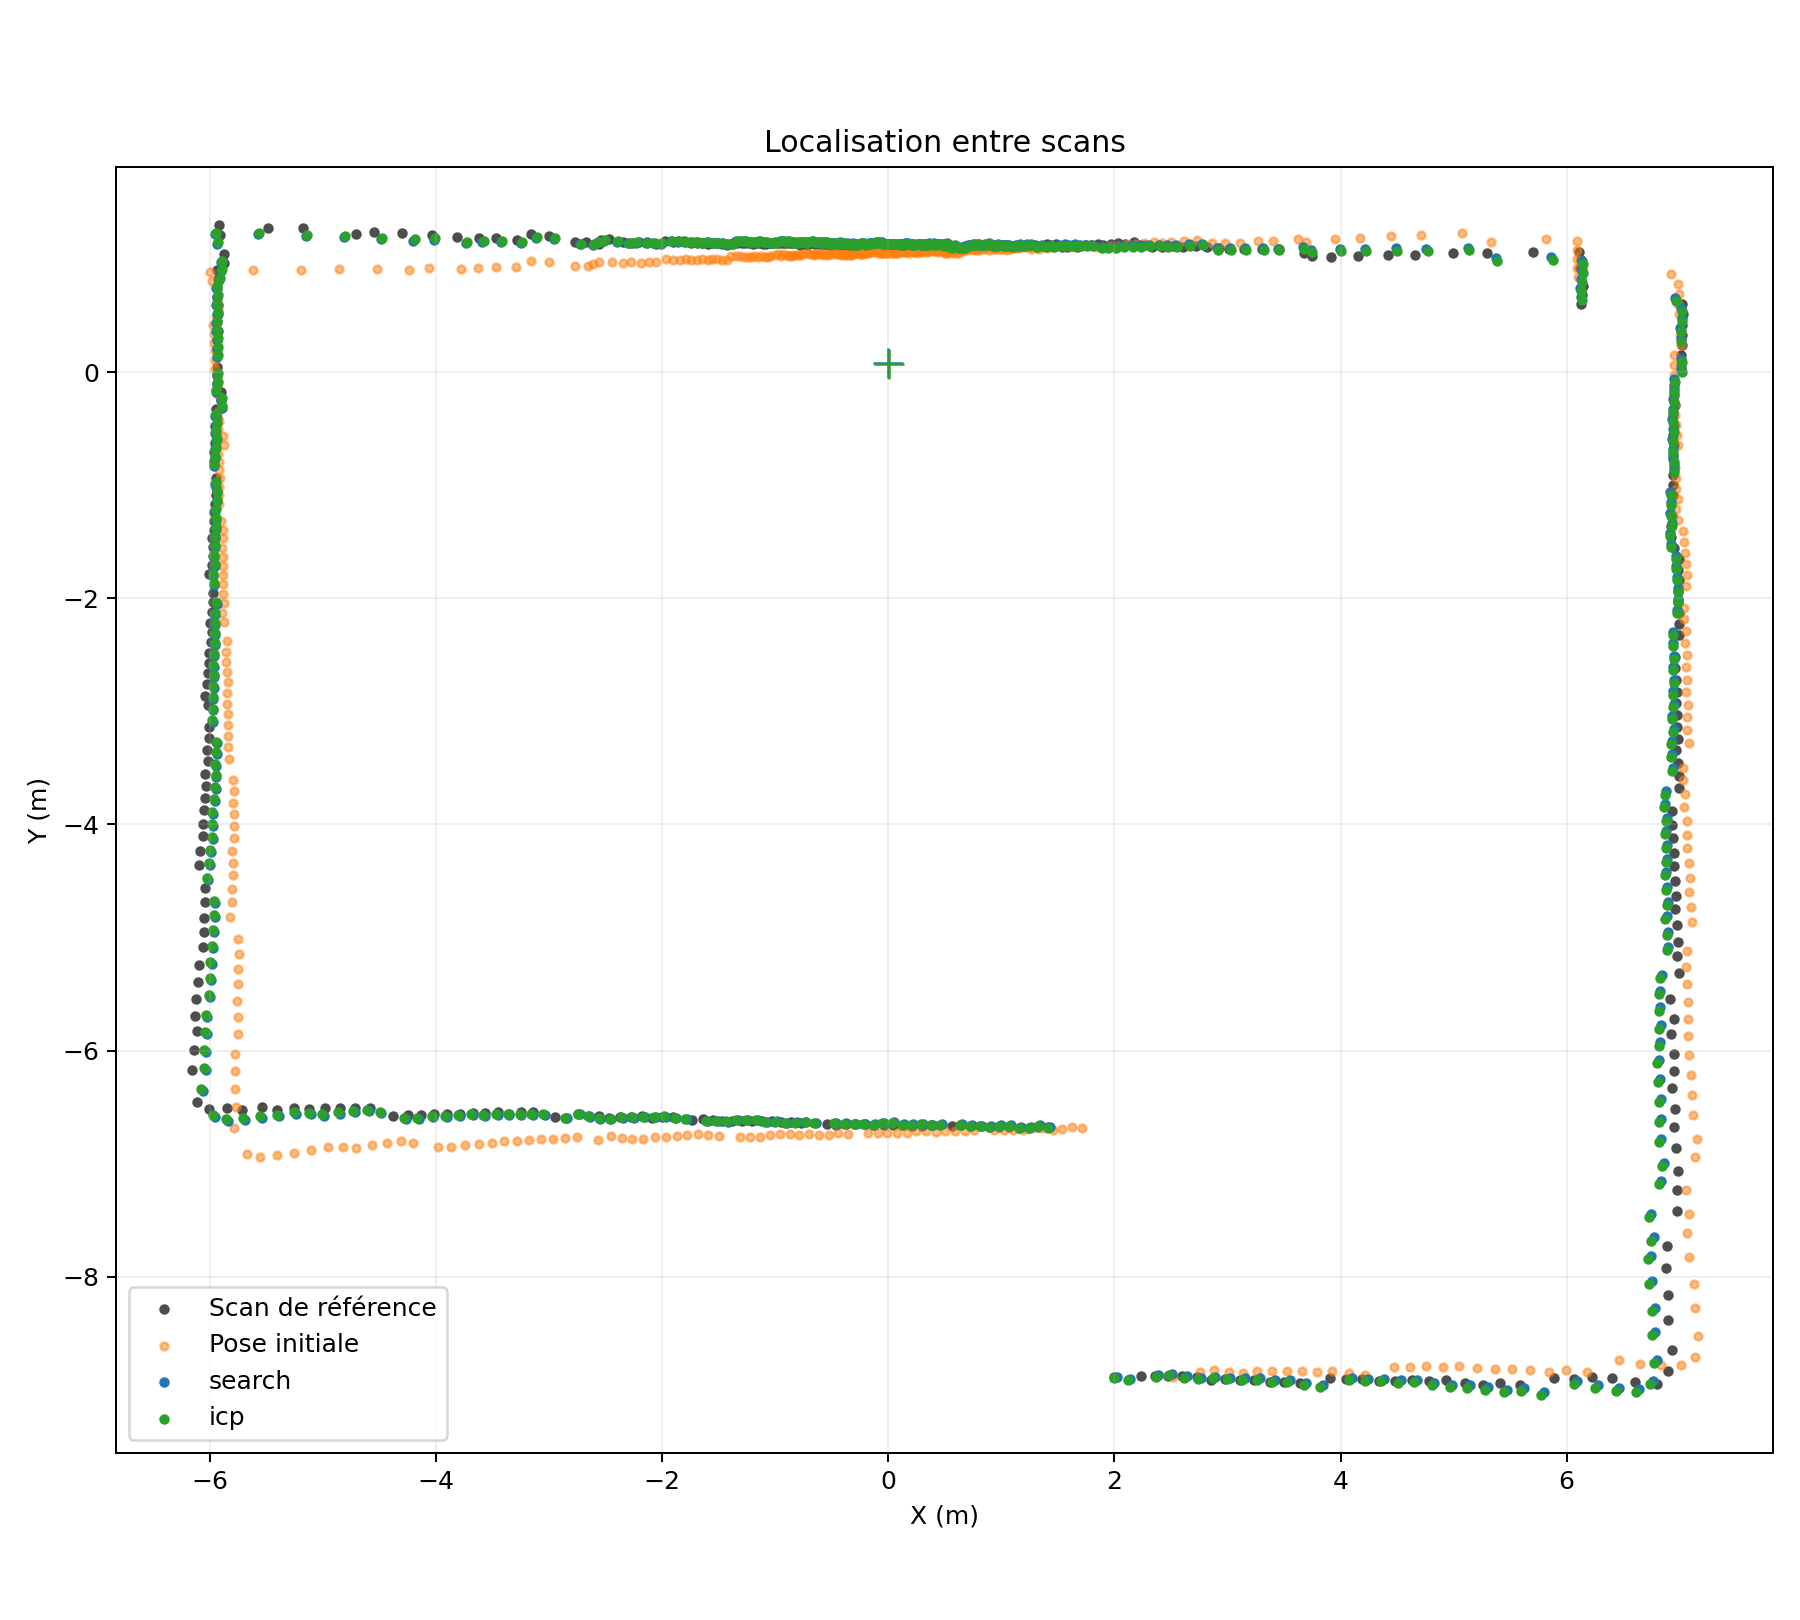
\includegraphics[width=0.82\linewidth]{localisation_scans_paire_2_3.png}
\caption{Paire réelle : Scan 3 dans le repère de Scan 2.
Gris : référence ; orange : placement initial ; bleu : recherche ;
vert : ICP. Les contours se superposent mieux après correction.}
\end{figure}

\subsection{Toutes les paires de Scan 1, Scan 2 et Scan 3}
L'outil \code{localisation_paires.py} complète les trois combinaisons :
Scan 2 vers Scan 1, Scan 3 vers Scan 1 et Scan 3 vers Scan 2.
Lorsque la pose relative initiale est inconnue, un amorçage ICP multidépart
est calculé. La recherche et l'ICP de raffinement reçoivent ensuite cette
\emph{même pose initiale estimée}. Le temps d'amorçage et les éventuelles
solutions alternatives sont conservés.

Ce protocole sert à produire un diagnostic visuel de chaque paire.
Puisque son amorçage utilise déjà l'ICP, il ne remplace pas la comparaison
indépendante à 144 essais avec initialisations imposées.

\begin{table}[htbp]
\centering
\caption{Poses candidates après raffinement ICP de toutes les paires réelles.}
\begin{tabular}{lrrrr}
\toprule
Transformation & $X$ (m) & $Y$ (m) & Angle & Recouvrement \\
\midrule
Scan 2 vers Scan 1 & $-0,378$ & $-2,431$ & $90,692^\circ$ & 67,0\,\% \\
Scan 3 vers Scan 1 & $-0,461$ & $-2,430$ & $178,166^\circ$ & 67,8\,\% \\
Scan 3 vers Scan 2 & 0,006 & 0,076 & $87,402^\circ$ & 99,8\,\% \\
\bottomrule
\end{tabular}
\end{table}

Les paires contenant Scan 1 partagent moins d'impacts proches de la
référence que la paire Scan 2/Scan 3. Les obstacles et les portions visibles
diffèrent. Les translations de l'ordre de 2,4 m par rapport à Scan 1 sont
des estimations et ne prouvent pas que les acquisitions respectent une
distance physique de proximité prédéfinie. L'alignement doit être vérifié
dans la salle ; les seuils de réussite sur poses connues ne sont pas
appliqués à ces paires sans vérité mesurée.

\begin{figure}[htbp]
\centering
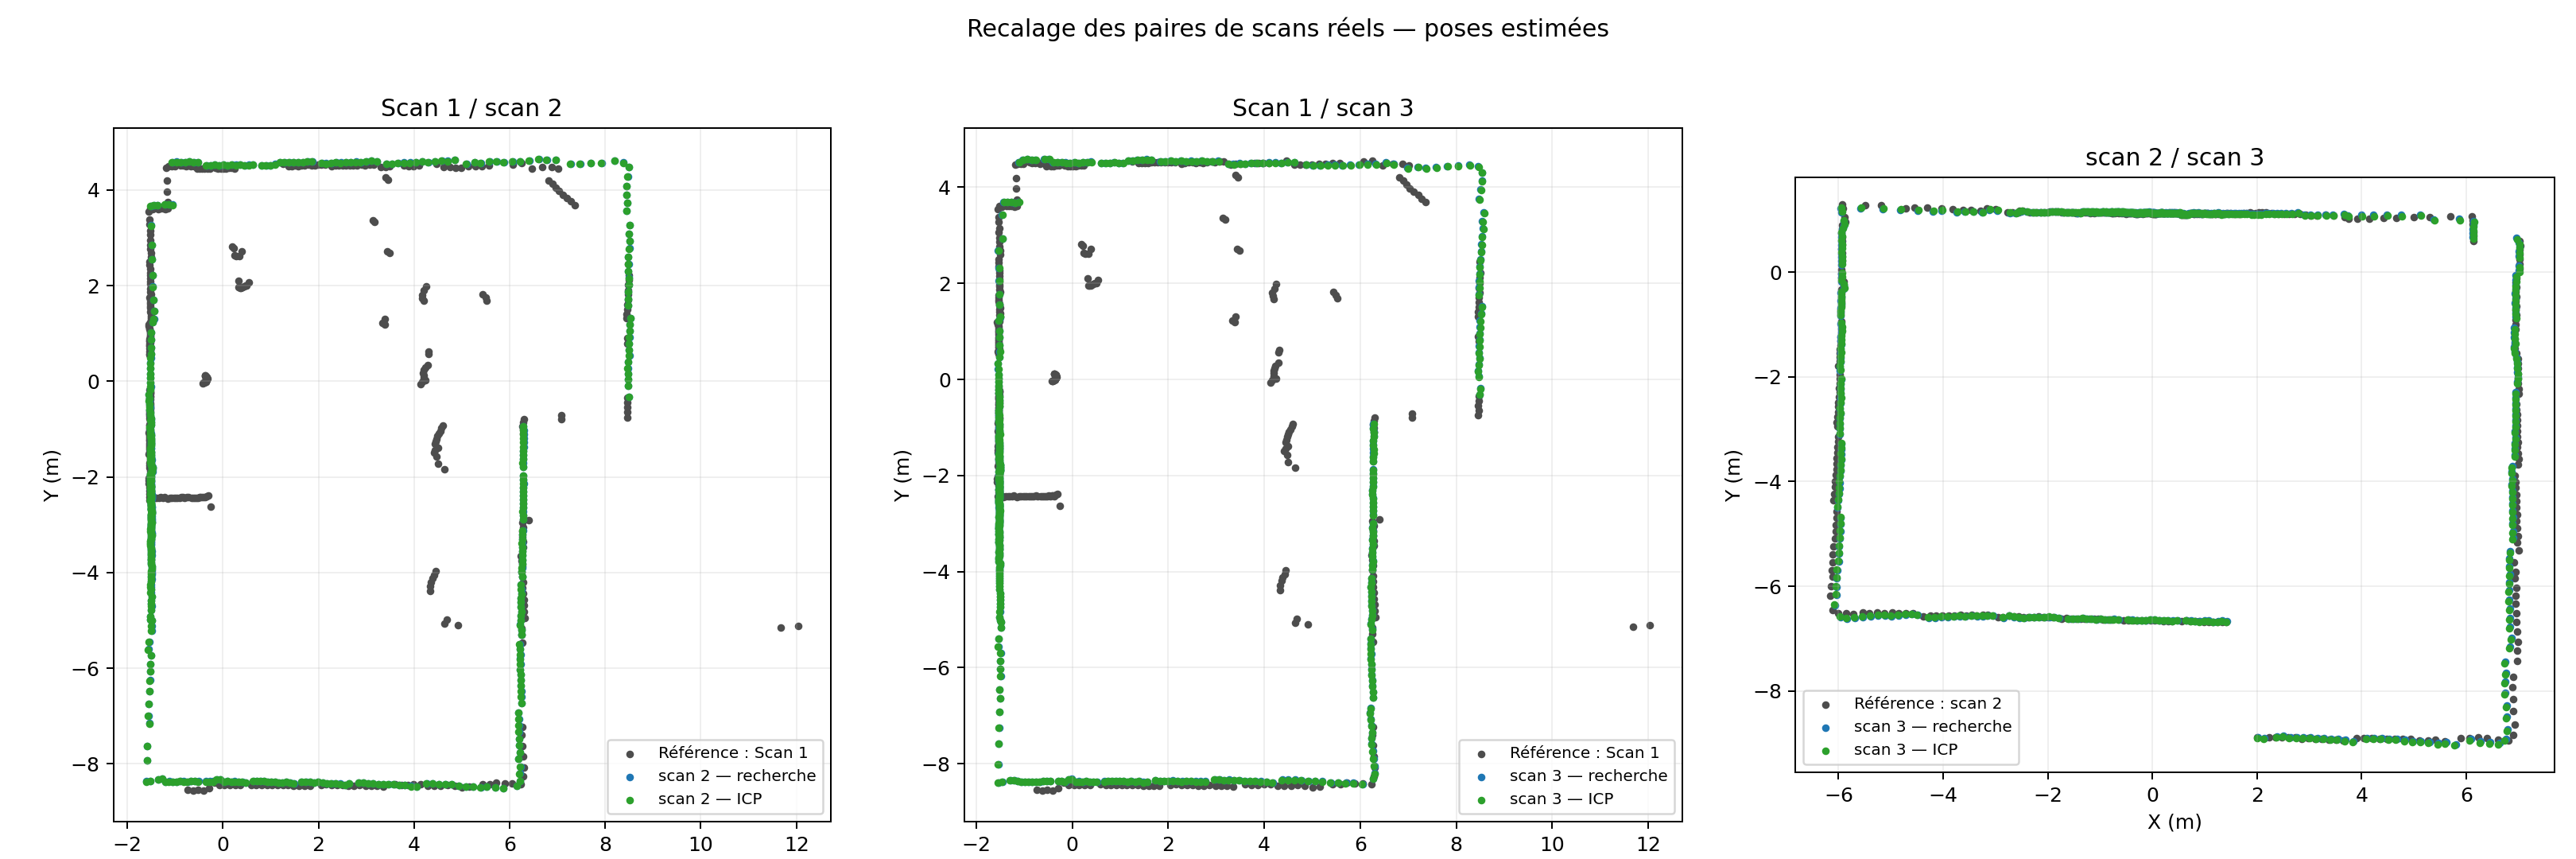
\includegraphics[width=\linewidth]{recalage_scans_reels.png}
\caption{Vue d'ensemble des trois paires réelles. Chaque panneau possède
son repère de référence : les positions ne sont pas directement comparables
d'un panneau à l'autre. Gris : référence ; bleu et vert : requête recalée.}
\end{figure}

\section{Version améliorée : bilan avant/après}\label{sec:amelioration}
\subsection{Effet mesuré des modifications}
Les deux campagnes utilisent exactement les mêmes requêtes, poses vraies et
initialisations ; seul le code de \code{localisation_scans.py} change.
La grille et la carte vectorielle ne sont pas modifiées et donnent des
résultats identiques.

\begin{table}[htbp]
\centering
\caption{Méthodes entre scans : erreurs moyennes de position (cm) et d'angle,
avant $\rightarrow$ après. Neuf essais par case ; 9/9 réussites partout.}
\begin{tabular}{lll}
\toprule
Données & Recherche entre scans & ICP entre scans \\
\midrule
Simulation & 1,08 $\rightarrow$ \textbf{0,80} ; $0,333^\circ\rightarrow\mathbf{0,267^\circ}$ & 0,85 $\rightarrow$ \textbf{0,68} ; $0,277^\circ\rightarrow\mathbf{0,111^\circ}$ \\
Scan 1 & 2,00 $\rightarrow$ \textbf{1,14} ; $0,800^\circ\rightarrow\mathbf{0,600^\circ}$ & 1,58 ; $0,775^\circ$ (inchangé) \\
Scan 2 & 5,18 $\rightarrow$ 5,51 ; $1,000^\circ$ (inchangé) & 2,94 ; $0,808^\circ$ (inchangé) \\
Scan 3 & 2,44 $\rightarrow$ \textbf{2,11} ; $0,800^\circ$ (inchangé) & 2,70 ; $0,807^\circ$ (inchangé) \\
\bottomrule
\end{tabular}
\end{table}

En simulation, l'ICP en deux phases divise l'erreur angulaire par 2,5.
Sur les points réels réservés, la recherche s'améliore sur Scan 1 et
Scan 3 mais se dégrade légèrement en position sur Scan 2 (+3 mm) ; l'ICP
garde ses valeurs, car la seconde phase n'abaisse pas le coût et sa pose
est rejetée. Le coût de calcul de l'ICP passe de 0,02 à 0,03--0,07 s.

\subsection{Artefact d'échantillonnage du protocole contrôlé}
La figure~\ref{fig:artefact} trace le coût d'un scan réel autour de la pose
vraie connue. Pour les trois mesures à base de points (champ de distance de
la grille, point-à-point et point-à-ligne), \emph{la pose vraie est un
maximum local} ; deux minima apparaissent vers $\pm0{,}8^\circ$, l'ordre de
grandeur du pas angulaire du LD06 ($0{,}73^\circ$ en médiane sur ce scan).

\begin{figure}[htbp]
\centering
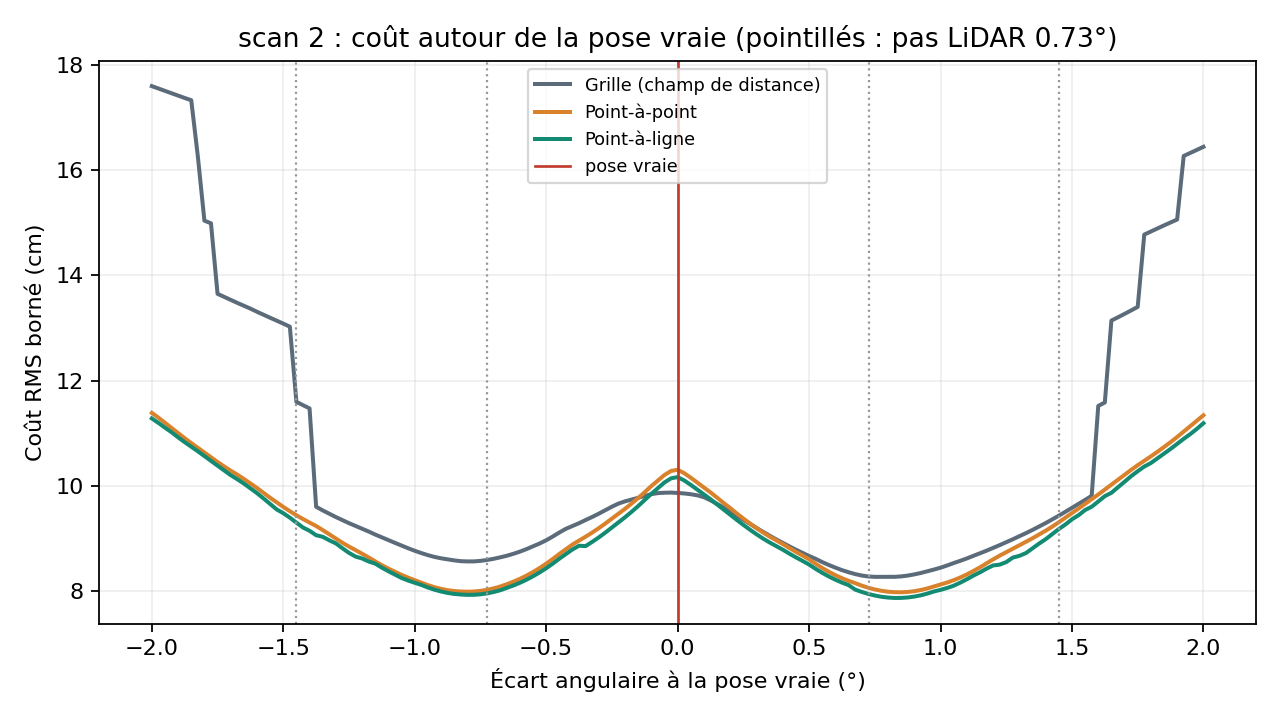
\includegraphics[width=0.85\linewidth]{artefact_echantillonnage.png}
\caption{Coût RMS borné de Scan 2 en fonction de l'écart angulaire à la
pose vraie (première pose du protocole). Les pointillés marquent les
multiples du pas angulaire du LiDAR.}
\label{fig:artefact}
\end{figure}

La référence (4 points sur 5) et le test (1 point sur 5) proviennent
\emph{du même scan} et partagent la même grille angulaire. Une rotation
d'environ un pas rapproche chaque point de test de points de référence
voisins, ce qui réduit le coût plus que la pose vraie elle-même. Les trois
méthodes à base de points convergent donc vers $\approx0{,}8^\circ$, avec des
valeurs presque identiques (l'ICP donne exactement $0{,}790^\circ$ sur Scan 2).
La carte vectorielle, qui mesure la distance à des segments ajustés,
n'est pas concernée ($0{,}0$ à $0{,}4^\circ$).

Conséquence : l'erreur angulaire des méthodes à base de points sur les
points réels réservés \emph{ne mesure pas leur précision réelle}. La distance
point-à-ligne ne supprime pas l'artefact, car seuls 52\,\% des points de
Scan 2 ont un voisinage rectiligne ; les autres gardent la distance
point-à-point. Entre deux acquisitions prises à des poses différentes,
les grilles angulaires ne coïncident pas et l'artefact disparaît :
c'est la situation des paires réelles et du SLAM du TP n° 3. Un protocole
plus juste réserverait des \emph{scans entiers} acquis à des poses mesurées.

\section{Incertitudes, validation et limites}
\subsection{Incertitude des références}
\begin{table}[htbp]
\centering
\caption{Portée des références et des erreurs calculées.}
\begin{tabularx}{\linewidth}{l>{\raggedright\arraybackslash}X>{\raggedright\arraybackslash}X}
\toprule
Protocole & Référence de pose & Incertitude et interprétation \\
\midrule
Simulation & Pose exacte définie dans le simulateur &
Pas d'incertitude de mesure physique de la pose ; bruit radial simulé de 5 mm \\
Points réels contrôlés & Transformation virtuelle connue &
Erreur de récupération géométrique ; aucune nouvelle pose physique mesurée \\
Paires réelles & Pose inconnue, estimée par recalage &
Incertitudes de position et d'angle non quantifiées ; résidu distinct de l'erreur de pose \\
\bottomrule
\end{tabularx}
\end{table}

Aucune position de référence métrique ni orientation exacte n'a été relevée
sur le robot pour les paires réelles. Il n'est donc pas possible d'annoncer
une borne de type « $\pm x$ cm » ou « $\pm y^\circ$ ». Les champs d'erreur
physique sont laissés vides dans les CSV et à \code{null} dans les JSON.
Les anciennes poses de fusion, elles-mêmes estimées par ICP, ne sont
pas utilisées comme vérité terrain physique.

Pour compléter l'évaluation sur robot, il faudra relever des poses proches
dans un repère commun, préciser les instruments et leur incertitude, puis
répéter des acquisitions immobiles. La comparaison pourra alors séparer
l'erreur de recalage, le bruit du capteur et l'incertitude de la référence.

\subsection{Validation logicielle}
La suite complète du projet comporte \textbf{74 tests réussis} lors de
la préparation de ce rapport. Les tests ajoutés pour le Jour 2 vérifient
notamment :
\begin{itemize}
\item les transformations de pose et le passage de $+180^\circ$ à $-180^\circ$ ;
\item les distances aux cellules, aux segments finis et aux points ;
\item le premier impact visible et la reproductibilité du bruit simulé ;
\item le raffinement ICP et l'absence de réflexion dans la transformation ;
\item l'identité des requêtes et des initialisations entre méthodes ;
\item la séparation entre points de référence et points réservés ;
\item le calcul du taux de réussite en conservant les échecs ;
\item le traitement des trois paires et l'absence de vérité terrain inventée.
\end{itemize}
Les scènes synthétiques de tests unitaires ne remplacent pas les essais
sur données réelles ; elles vérifient des comportements géométriques connus.

\subsection{Limites des résultats}
Une salle rectangulaire peut présenter des alignements concurrents.
Les objets mobiles, les surfaces cachées et les dédoublements de murs
affectent les trois représentations. La grille peut accumuler des
observations contradictoires ; la carte vectorielle peut conserver des
segments doublés ou écarter de petits objets ; le recalage entre scans
reste sensible à la densité et aux surfaces communes.

La campagne ne couvre qu'une scène simulée, un niveau de bruit et un
ensemble limité d'initialisations. Les valeurs de temps correspondent
à une exécution sur le poste utilisé et ne constituent pas une étude
statistique de performance. Les scores résiduels des différentes
références ne sont pas directement équivalents : la comparaison utilise
les erreurs de pose connues, les durées et les taux de réussite.

\section*{Conclusion}
\addcontentsline{toc}{section}{Conclusion}
Les trois volets du TP disposent d'outils fonctionnels : localisation sur
grille d'occupation, sur carte vectorielle et entre scans. Deux méthodes
ont été développées pour ce dernier volet, une recherche hiérarchique et
un ICP. Dans la version améliorée, toutes deux utilisent la distance au mur
local (point-à-ligne) et l'ICP fonctionne en deux phases ; l'erreur angulaire
simulée de l'ICP passe de $0{,}277^\circ$ à $0{,}111^\circ$, et les deux méthodes
s'accordent à $0{,}2^\circ$ près sur la paire réelle Scan 2/Scan 3.

La comparaison commune de 144 essais utilise les mêmes requêtes et les
mêmes poses initiales pour toutes les méthodes. Dans la plage étudiée,
elles respectent toutes les seuils de 0,10 m et $1^\circ$ ; l'ICP est le
plus rapide sur ces données. L'erreur d'environ $0{,}8^\circ$ commune aux
méthodes à base de points sur les points réels réservés est un artefact
d'échantillonnage du protocole, démontré par le tracé du coût. Les campagnes exploratoires révèlent aussi
les difficultés de la grille fusionnée, conservées dans les résultats.

Les trois paires des acquisitions réelles ont été recalées et visualisées.
L'étape suivante pour une validation physique est de mesurer des poses de
référence et leurs incertitudes, puis d'élargir les essais aux
initialisations difficiles, aux symétries et aux changements de scène.

\clearpage
\appendix
\section{Organisation des outils et reproduction}
\begin{itemize}
\item \code{localisation_grid.py} : recherche sur champ de distance.
\item \code{localisation_vectorielle.py} : distance aux segments.
\item \code{localisation_scans.py} : recherche entre scans et ICP.
\item \code{comparaison_localisation.py} : simulation et campagne commune.
\item \code{localisation_paires.py} : traitement des paires réelles.
\end{itemize}
Les calculs utilisent notamment NumPy et SciPy, les figures Matplotlib,
la lecture Excel OpenPyXL et les tests Pytest. L'environnement utilisé
pour les validations est Python 3.9.6.

\begin{lstlisting}
python -m pip install -r requirements.txt
python -m pytest -q

cd version_amelioree
python comparaison_localisation.py --scans \
  "donnees/Scan 1.xlsx" "donnees/scan 2.xlsx" "donnees/scan 3.xlsx"

python localisation_scans.py "donnees/scan 2.xlsx" "donnees/scan 3.xlsx" \
  --initial 0 0 90 --output resultats/paire_2_3

python localisation_paires.py \
  "donnees/Scan 1.xlsx" "donnees/scan 2.xlsx" "donnees/scan 3.xlsx"

python figures_ameliorees.py   # tracé de l'artefact d'échantillonnage
\end{lstlisting}
Les commandes s'exécutent depuis le dossier \code{version_amelioree}.
La comparaison sans option \code{--scans} évalue uniquement la simulation.

Les principales sorties sont :
\begin{itemize}
\item le CSV détaillé des 144 essais, le résumé CSV/Markdown et le JSON
du protocole ;
\item le CSV par niveau d'initialisation et les courbes de sensibilité ;
\item les références, requêtes et poses connues dans les NPZ numériques ;
\item les images et diagnostics JSON des paires réelles.
\end{itemize}
Les résultats du rapport sont issus des fichiers exportés ; les classeurs
originaux restent inchangés.

\section{Ressources et traçabilité}
\begin{itemize}
\item Consignes du TP Jour 2 fournies : trois types de référence,
comparaison, sensibilité à l'initialisation et incertitudes.
\item Scans réels et cartes construits au TP n° 1.
\item Métadonnées JSON, résultats CSV et tests du projet.
\item Simulation par lancer de rayons documentée dans le code.
\end{itemize}
Le code et les résultats publiés sont accessibles dans le dépôt :

\url{https://github.com/sipsiploopcup/TP-Adib}.

Le rapport sépare explicitement résultats simulés, changements de repère
contrôlés et recalages physiques non étalonnés.

\end{document}
